%%%%%%%%%%%%%%%%%%%%%%%%%%%%%%%%%%%%%%%%%%%%%%%%%%%%%%%%%%%%
%%  This Beamer template was created by Cameron Bracken.
%%  Anyone can freely use or modify it for any purpose
%%  without attribution.
%%
%%  Last Modified: January 9, 2009
%%

\documentclass[xcolor=x11names,compress,8pt,fleqn]{beamer}
%\documentclass[xcolor=x11names,compress,8pt,handout]{beamer}

%%% langue
\usepackage[francais]{babel}

\usepackage[T1]{fontenc}
\usepackage[utf8]{inputenc}

%%% mathématiques
\usepackage{amsmath,amsfonts,amssymb,newlfont,latexsym}

 \def\leq{\leqslant}
 \def\geq{\geqslant}
 
 \def\real{\mathbb{R}}
 \def\Prob{\mathbb{P}}
 
 \def\integer{\mathbb{N}}
 \def\relative{\mathbb{Z}}
 \def\Esp{\mathbb{E}}
 
%%%%% algorithmes
\usepackage[vlined]{algorithm2e}

\SetKw{KwDownTo}{downto}
\SetKwIF{If}{ElseIf}{Else}{if}{}{else if}{else}{endif}
\SetKwFor{For}{for}{}{endfor}
\SetKwFor{While}{while}{}{endw}%

\SetKwInput{KwIn}{Input}%
\SetKwInput{KwOut}{Output}%
\SetKwInput{KwData}{Données}%
\SetKwInput{KwResult}{Résultats}%

%%%%% hyperliens
\usepackage{hyperref,url}
\hypersetup{
dvips,
backref=true, %permet d'ajouter des liens dans...
pagebackref=true,%...les bibliographies
hyperindex=true, %ajoute des liens dans les index.
colorlinks=true, %colorise les liens
breaklinks=true, %permet le retour à la ligne dans les liens trop longs
urlcolor= Blue4, %couleur des hyperliens
linkcolor= Blue4, %couleur des liens internes
bookmarks=true, %créé des signets pour Acrobat
bookmarksopen=true} 

%% General document %%%%%%%%%%%%%%%%%%%%%%%%%%%%%%%%%%
\usepackage{graphicx}
\graphicspath{{logos/}{images/}{figures/}{photos/}}
\usepackage{figlatex}%

\definecolor{gris05}{gray}{0.95}



\usepackage{tikz}
\usepackage{pgfplots}

%\usetikzlibrary{decorations.fractals}
%%%%%%%%%%%%%%%%%%%%%%%%%%%%%%%%%%%%%%%%%%%%%%%%%%%%%%
%% Beamer Layout %%%%%%%%%%%%%%%%%%%%%%%%%%%%%%%%%%
\useoutertheme[subsection=false,shadow]{miniframes}
\useinnertheme{default}
%\usefonttheme{serif}
\usepackage{palatino}

\setbeamerfont{title like}{shape=\scshape}
\setbeamerfont{frametitle}{shape=\scshape}

\setbeamercolor*{lower separation line head}{bg=DeepSkyBlue4} 
\setbeamercolor*{normal text}{fg=black,bg=white} 
\setbeamercolor*{alerted text}{fg=IndianRed4} 
\setbeamercolor*{example text}{fg=Green4} 
\setbeamercolor*{structure}{fg=black} 
 
\setbeamercolor*{palette tertiary}{fg=black,bg=black!10} 
\setbeamercolor*{palette quaternary}{fg=black,bg=black!10} 

%\setbeamertemplate{itemize item}{\scriptsize\raise1.25pt\hbox{\donotcoloroutermaths$\blacktriangleright$}}
%\setbeamertemplate{itemize subitem}{\tiny\raise1.5pt\hbox{\donotcoloroutermaths$\blacktriangleright$}}
%\setbeamertemplate{itemize subsubitem}{\tiny\raise1.5pt\hbox{\donotcoloroutermaths$\blacktriangleright$}}
%\setbeamertemplate{enumerate item}{\insertenumlabel.}
%\setbeamertemplate{enumerate subitem}{\insertenumlabel.\insertsubenumlabel}
%\setbeamertemplate{enumerate subsubitem}{\insertenumlabel.\insertsubenumlabel.\insertsubsubenumlabel}
%\setbeamertemplate{enumerate mini template}{\insertenumlabel}


\renewcommand{\(}{\begin{columns}}
\renewcommand{\)}{\end{columns}}
\newcommand{\<}[1]{\begin{column}{#1}}
\renewcommand{\>}{\end{column}}
%%%%%%%%%%%%%%%%%%%%%%%%%%%%%%%%%%%%%%%%%%%%%%%%%%
\usefonttheme{progressbar}
\useoutertheme{progressbar}
\useinnertheme{progressbar}


\setbeamertemplate{itemize item}[triangle]  
\setbeamertemplate{itemize subitem}[triangle]  
\setbeamertemplate{enumerate item}[diamond] 

\setbeamertemplate{navigation symbols}{}

%\beamertemplatetransparentcovereddynamic

% \setbeamercovered{transparent}

\pgfdeclareimage[height=0.5cm]{university-logo}{logos/logoUGA.jpg}
  
\logo{\pgfuseimage{university-logo}}

\title[Représentation des données] % (optional, use only with long paper titles)
{Représentation des données}
\subtitle{Checklist for good graphics}

\author% (optional, use only with lots of authors)
{
\textbf{Jean-Marc.Vincent}@imag.fr	
}
% - Give the names in the same order as the appear in the paper.
% - Use the \inst{?} command only if the authors have different
%   affiliation.

\institute[Université de Grenoble-Alpes] % (optional, but mostly needed)
{%

\includegraphics[width=1.5cm]{logos/logo_UFR_IM2AG.jpg}
}
% - Use the \inst command only if there are several affiliations.
% - Keep it simple, no one is interested in your street address.

\date[Grenoble] % (optional, should be abbreviation of conference name)
{
Grenoble 2017\\
MIAGE
}



% \AtBeginSection[]
%{
%  \begin{frame}<beamer>
%    \frametitle{Complexité de problèmes}
%    \tableofcontents[currentsection]
%  \end{frame}
%}

\begin{document}

\begin{frame}
\titlepage
\end{frame}
\begin{frame}
    \frametitle{Principes pour la visualisation}
    \tableofcontents
  \end{frame}
  \section[{\scshape Problème}]{{\scshape Problème :} Représentation des données}
\begin{frame}{La présentation}
\begin{block}{Problème : fournir de jolies images pour aider à la compréhension}
\begin{itemize}
\item \alert{\bf Améliorer grandement la qualité d'un article}

\item Montrer la qualité de votre travail

\item Les images/figures/diagrammes entrainent des discussions

\item et génèrent de nouveaux problèmes
\end{itemize}
\end{block}
\begin{block}{Erreurs de présentation}
\begin{itemize}
\item \alert{\bf Sémantique des objets graphiques}
\item conventions pour les schémas/diagrammes... 
\item premiers pas vers la validation
\end{itemize}
\end{block}
\end{frame}
 \section[{\scshape Guidelines}]{{\scshape Principes :} Idées de base}
%\begin{frame}{Guidelines for good graphics (Jain)}
%\begin{block}{Guidelines for Preparing Good Graphic Charts}
%\alert{\bf Specify the amount of information given by the chart}
%\begin{enumerate}
%\item  Require Minimum Effort from the Reader
%\item Maximize Information
%\item Minimize Ink
%\item  Use Commonly Accepted Practices
%\item  Make several trials before arriving at the final chart. Different combinations should be tried and the best
%one selected.
%\end{enumerate}
%\end{block}
%\end{frame}
\begin{frame}{Guidelines for good graphics (Jain)}
\begin{block}{Minimum effort for the reader}
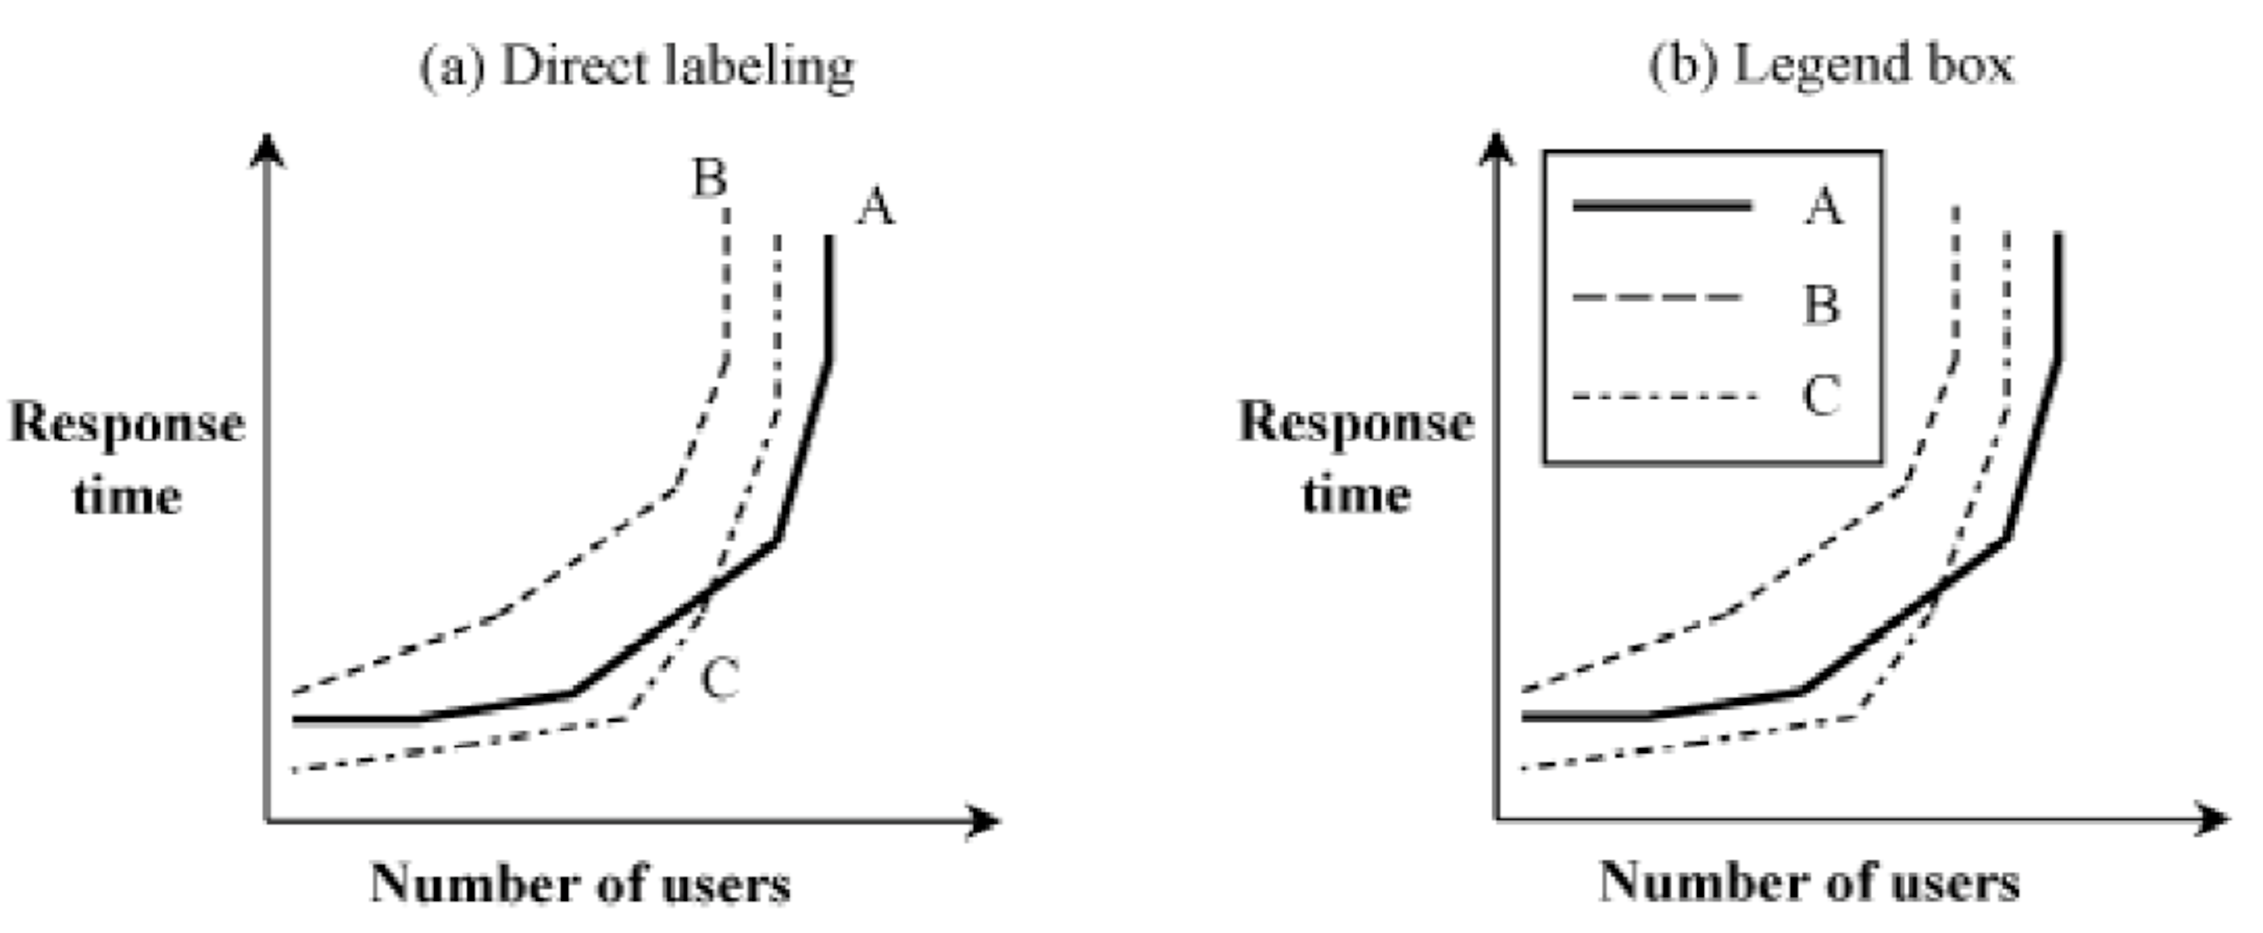
\includegraphics[width=10.8cm]{Jain-graph1}
\end{block}
\end{frame}
\begin{frame}{Guidelines for good graphics (Jain)}
\begin{block}{Minimize Ink}
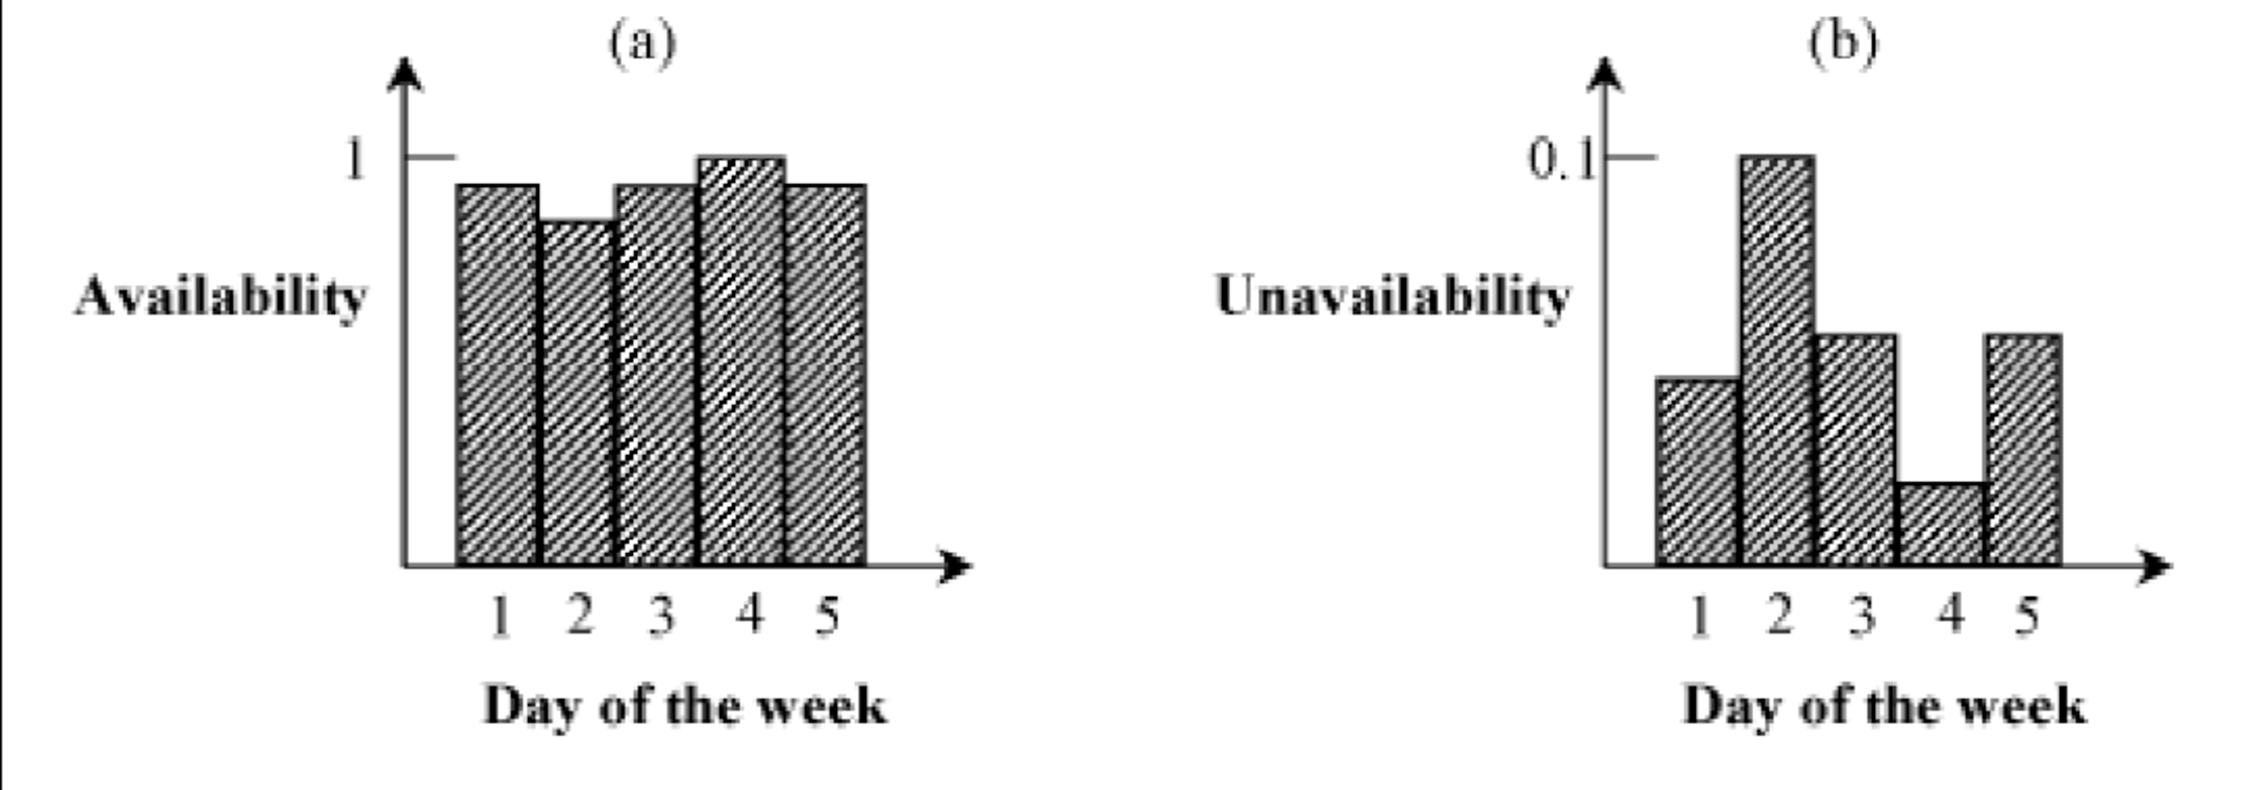
\includegraphics[width=10.8cm]{Jain-graph2}
\end{block}
\end{frame}
\section{Common Mistakes}
\begin{frame}{Common mistakes}
\begin{block}{Multiple scaling, Too much information}
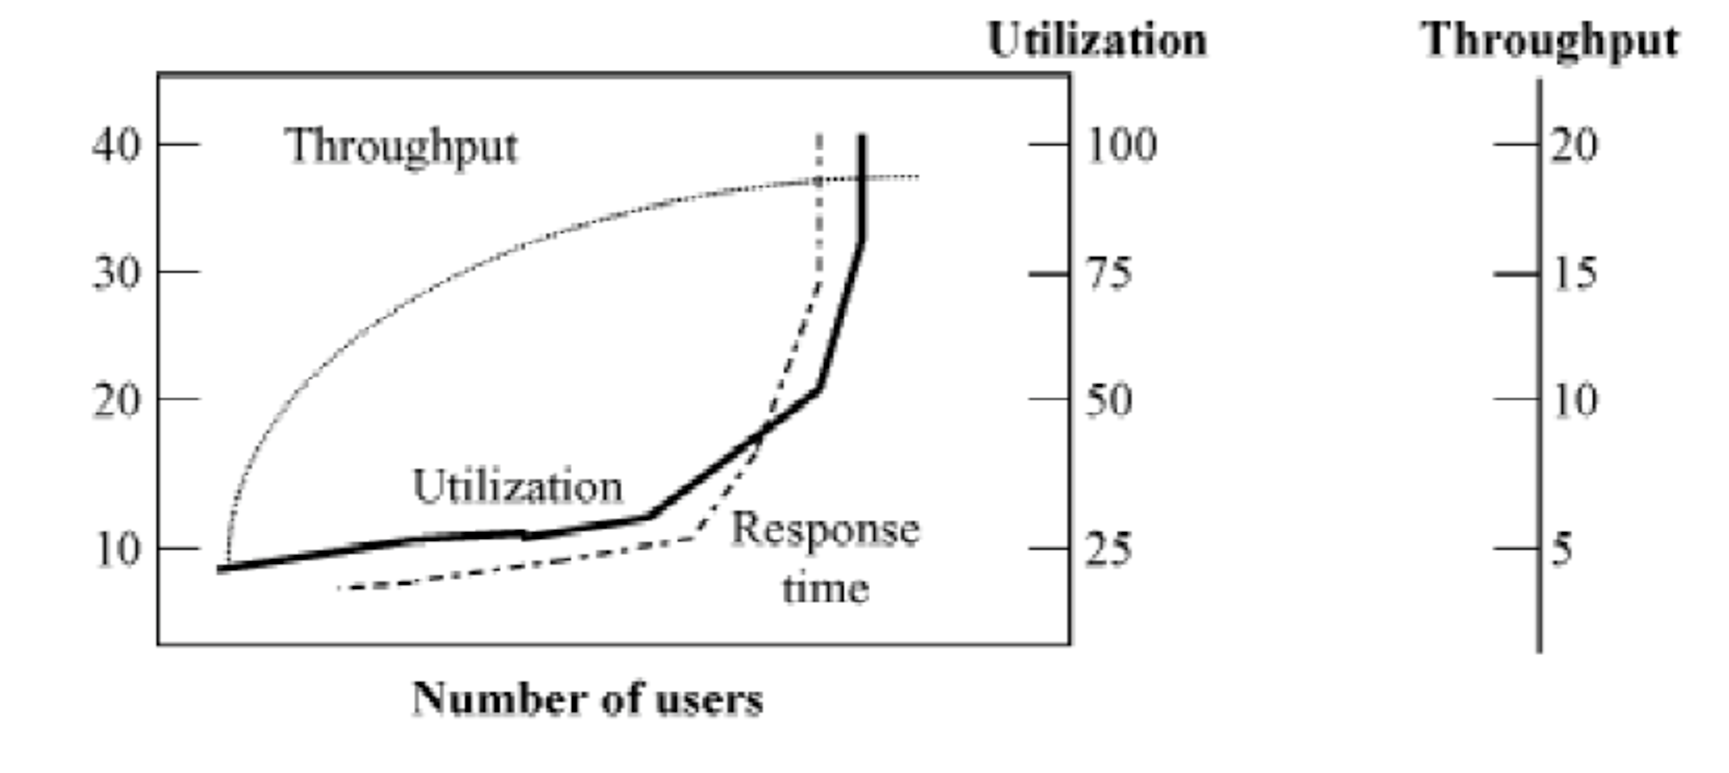
\includegraphics[width=10.8cm]{Jain-graph3}
\end{block}
\end{frame}
\begin{frame}{Common mistakes}
\begin{block}{Cryptic information}
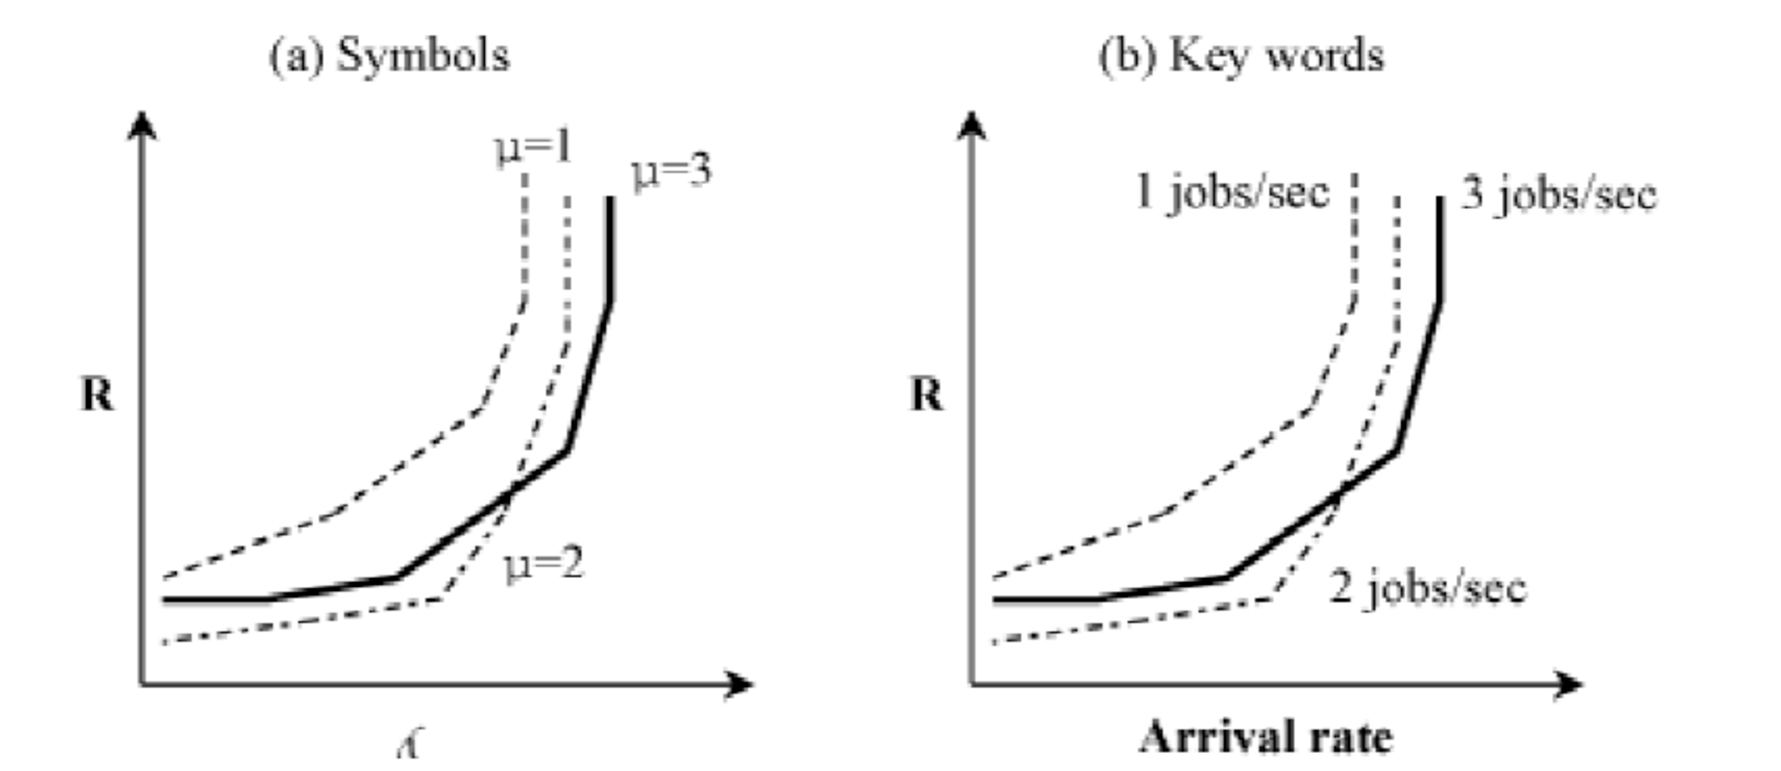
\includegraphics[width=10.8cm]{Jain-graph4}
\end{block}
\end{frame}
\begin{frame}{Common mistakes}
\begin{block}{Non-relevant graphic objects}
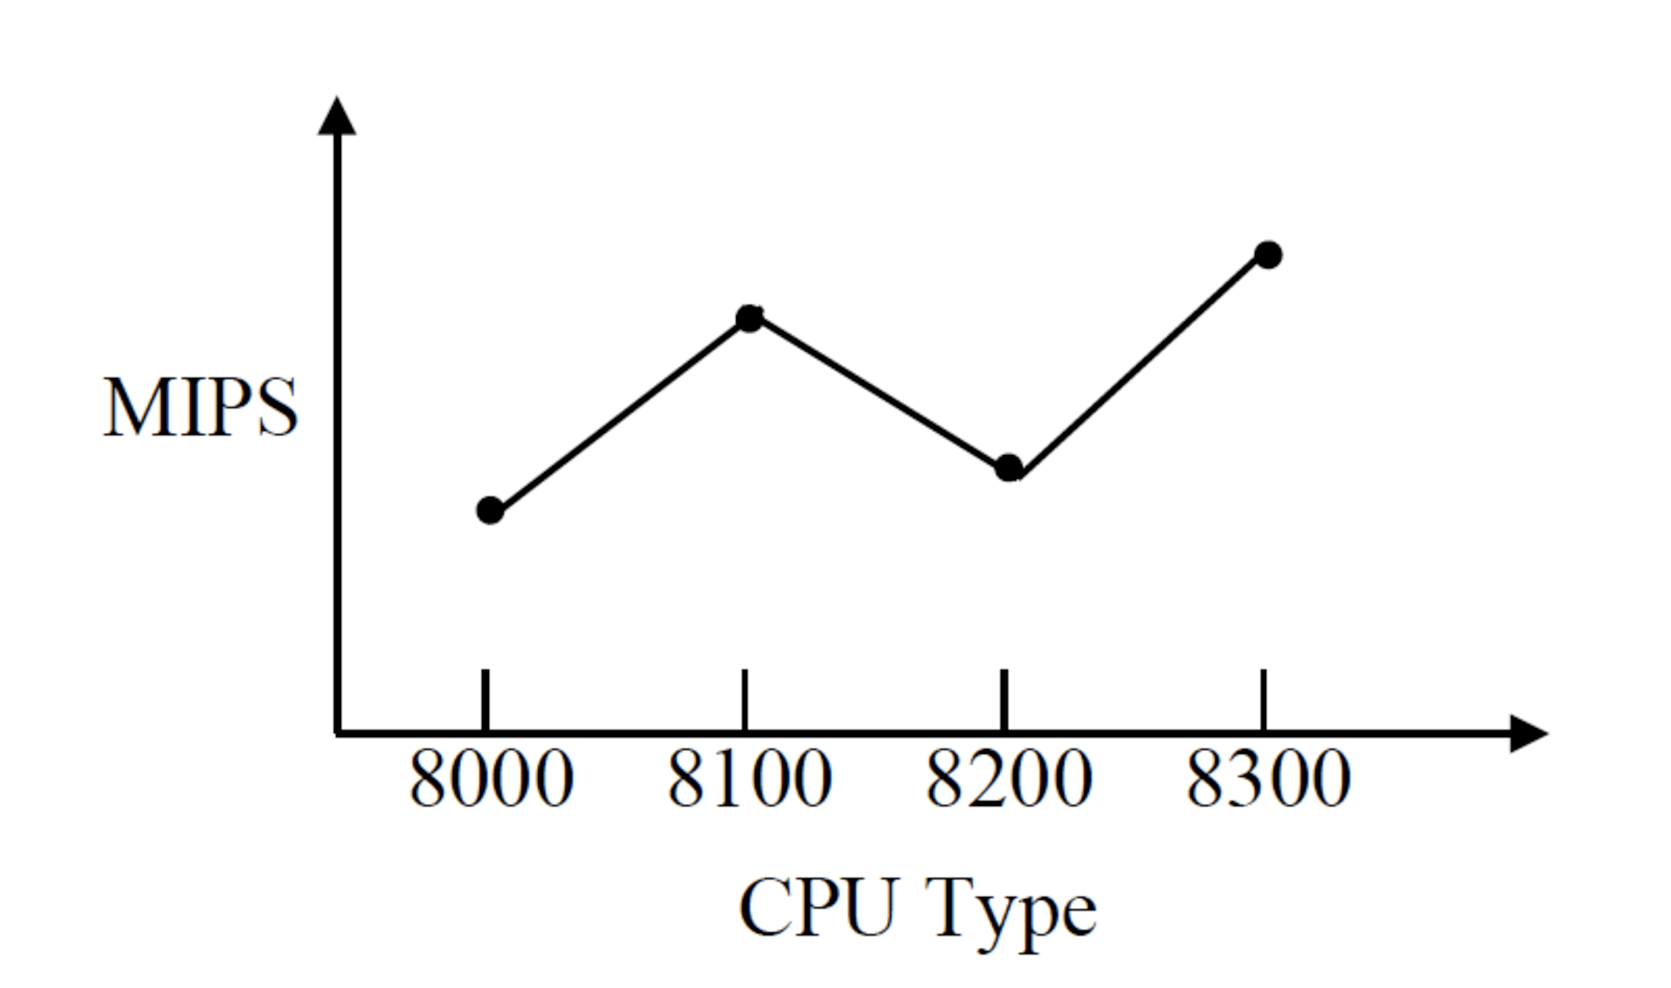
\includegraphics[width=10.8cm]{Jain-graph5}
\end{block}
\end{frame}
\begin{frame}{Common mistakes}
\begin{block}{Non-relevant graphic objects}
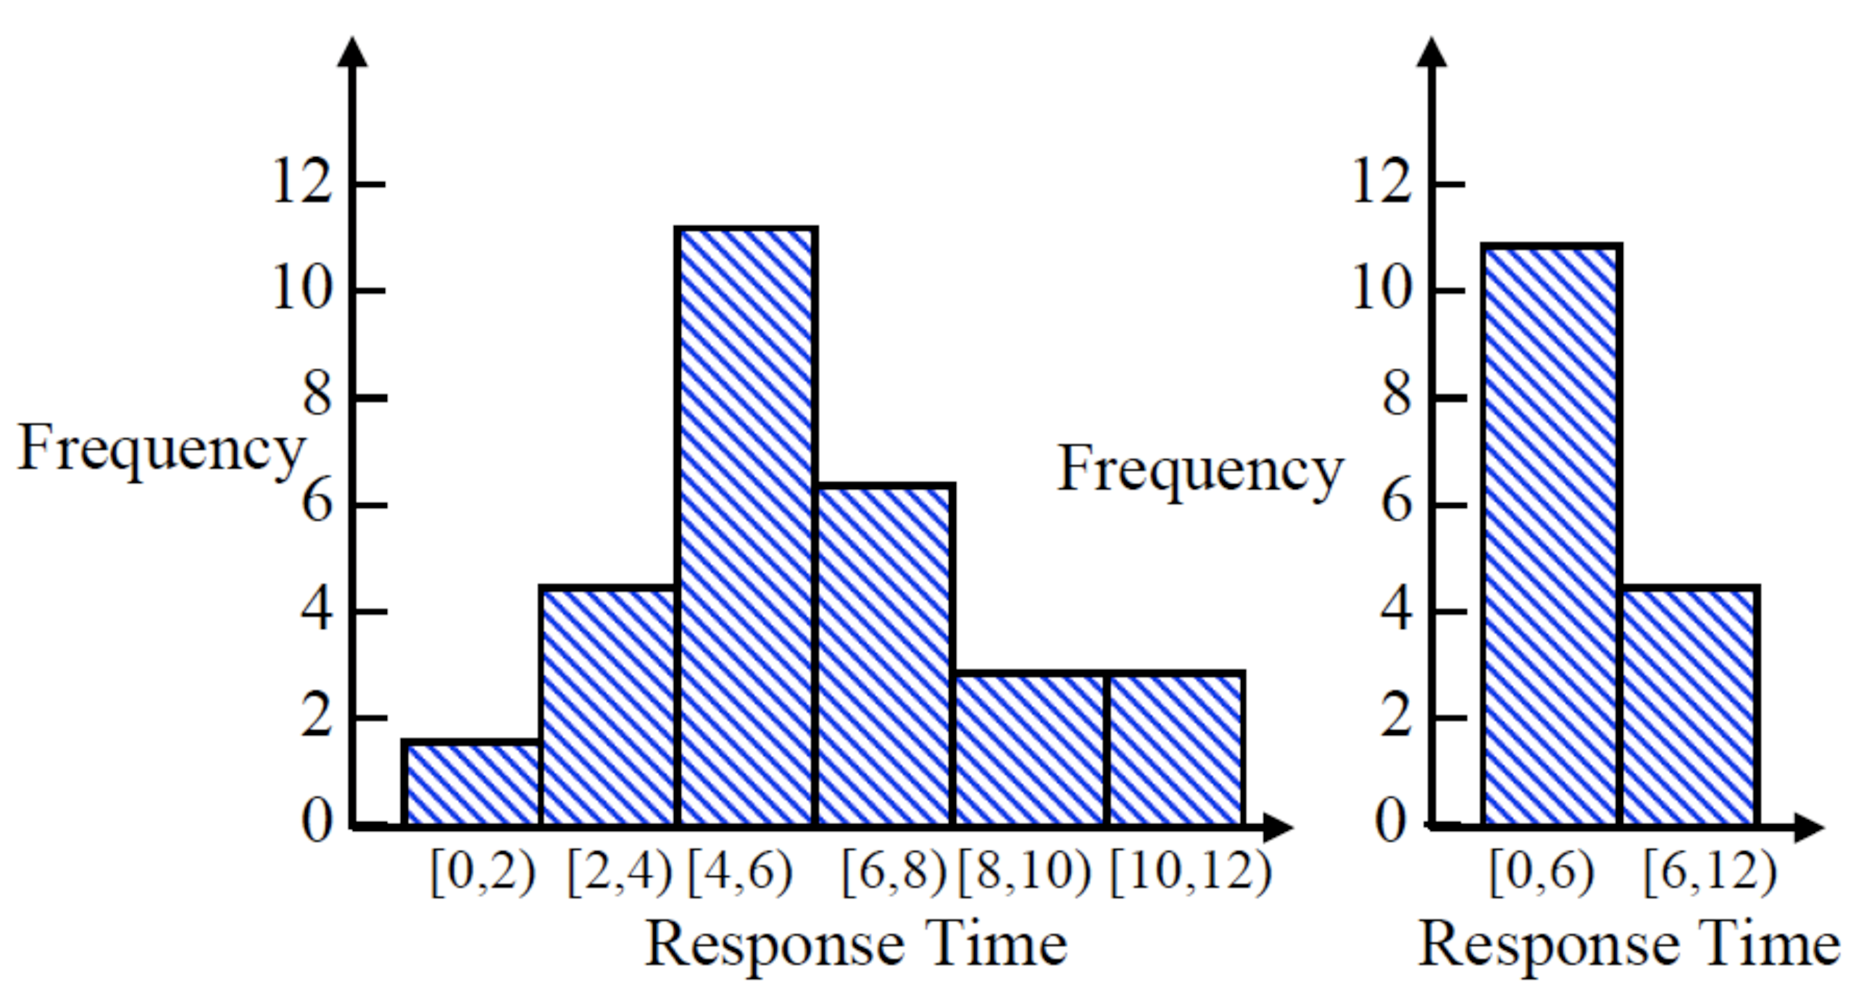
\includegraphics[width=10.8cm]{Jain-graph8}
\end{block}
\end{frame}
\begin{frame}{Common mistakes}
\begin{block}{Howto cheat ?}
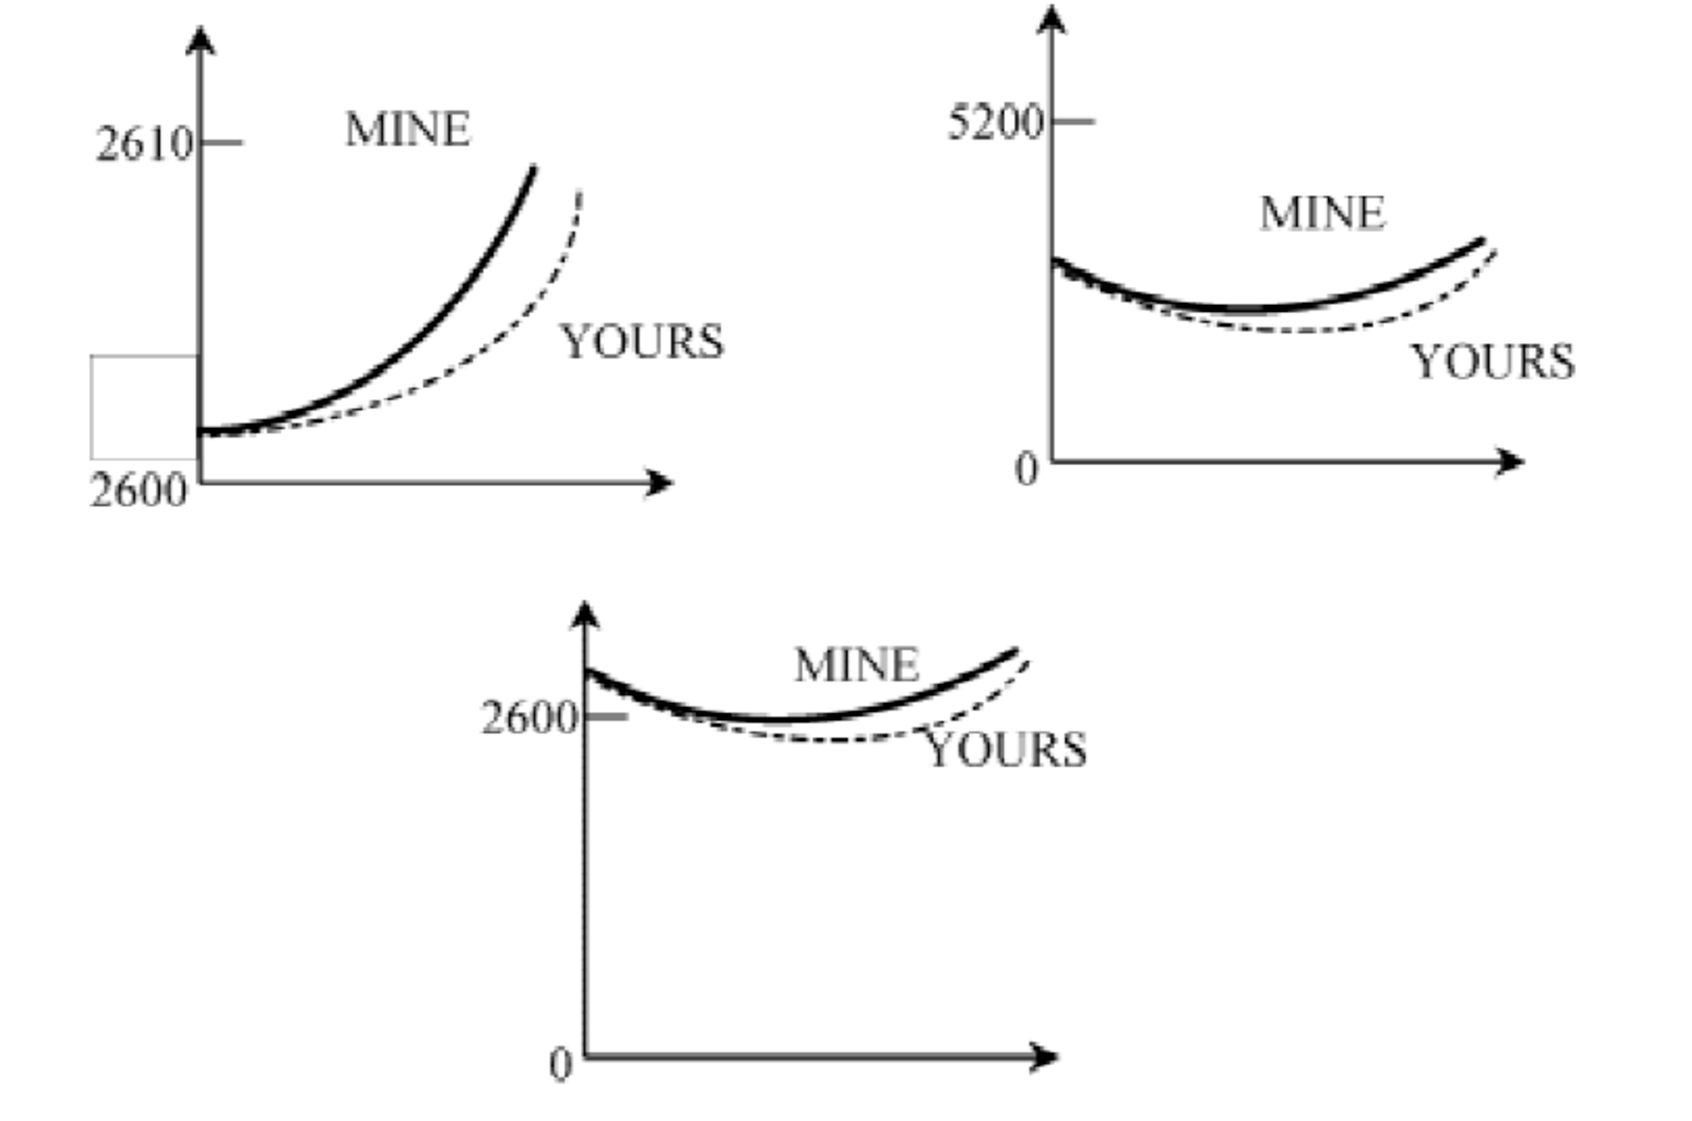
\includegraphics[width=10.8cm]{Jain-graph6}
\end{block}
\end{frame}
\begin{frame}{Common mistakes}
\begin{block}{Howto cheat ?}
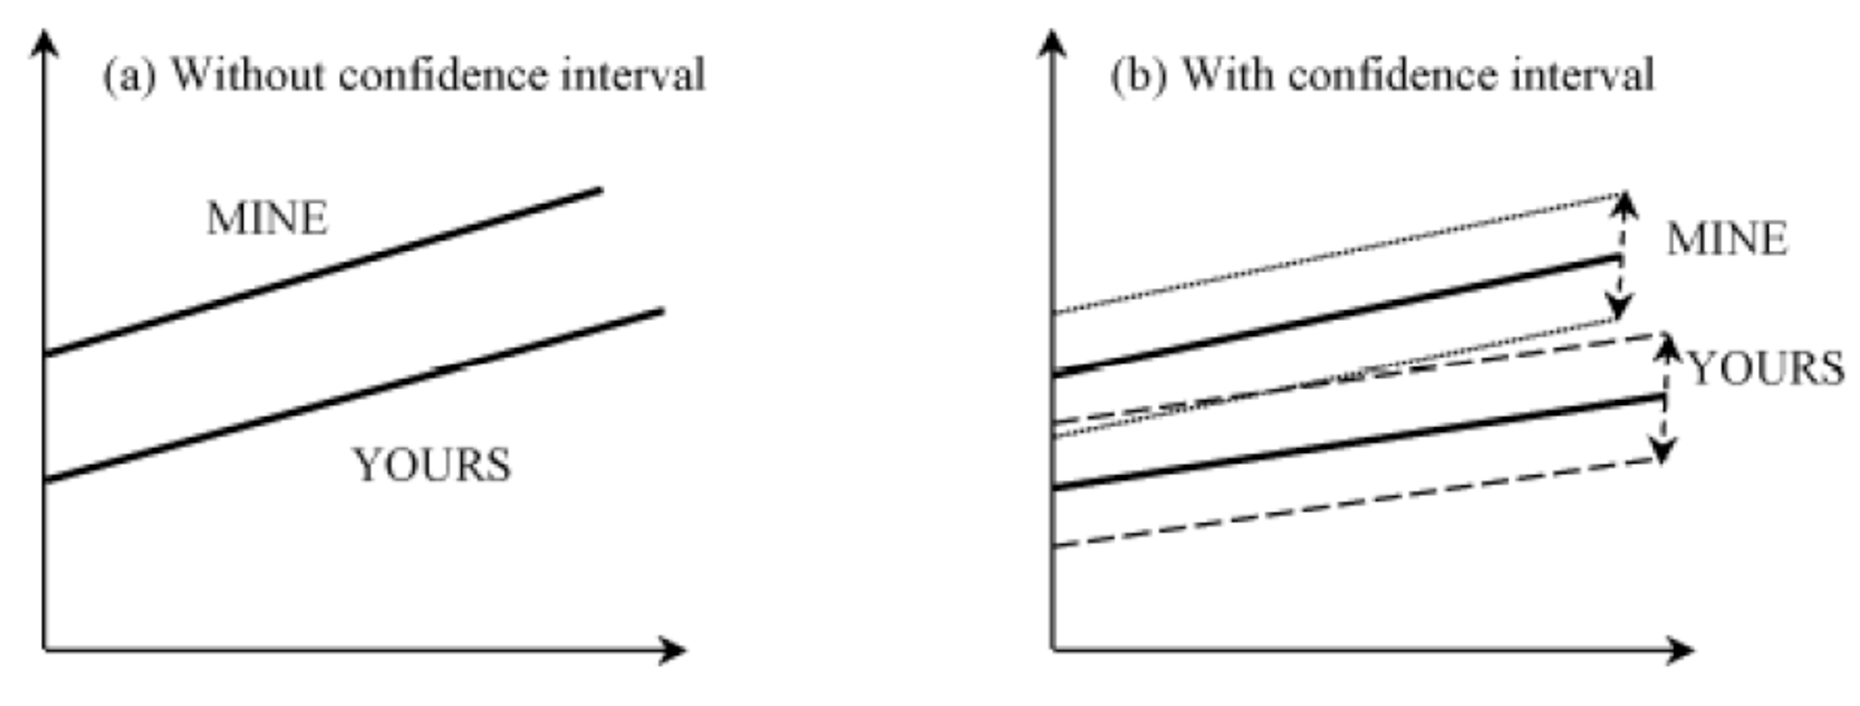
\includegraphics[width=10.8cm]{Jain-graph7}
\end{block}
\end{frame}
\begin{frame}{Common mistakes}
\begin{block}{Howto cheat ?}
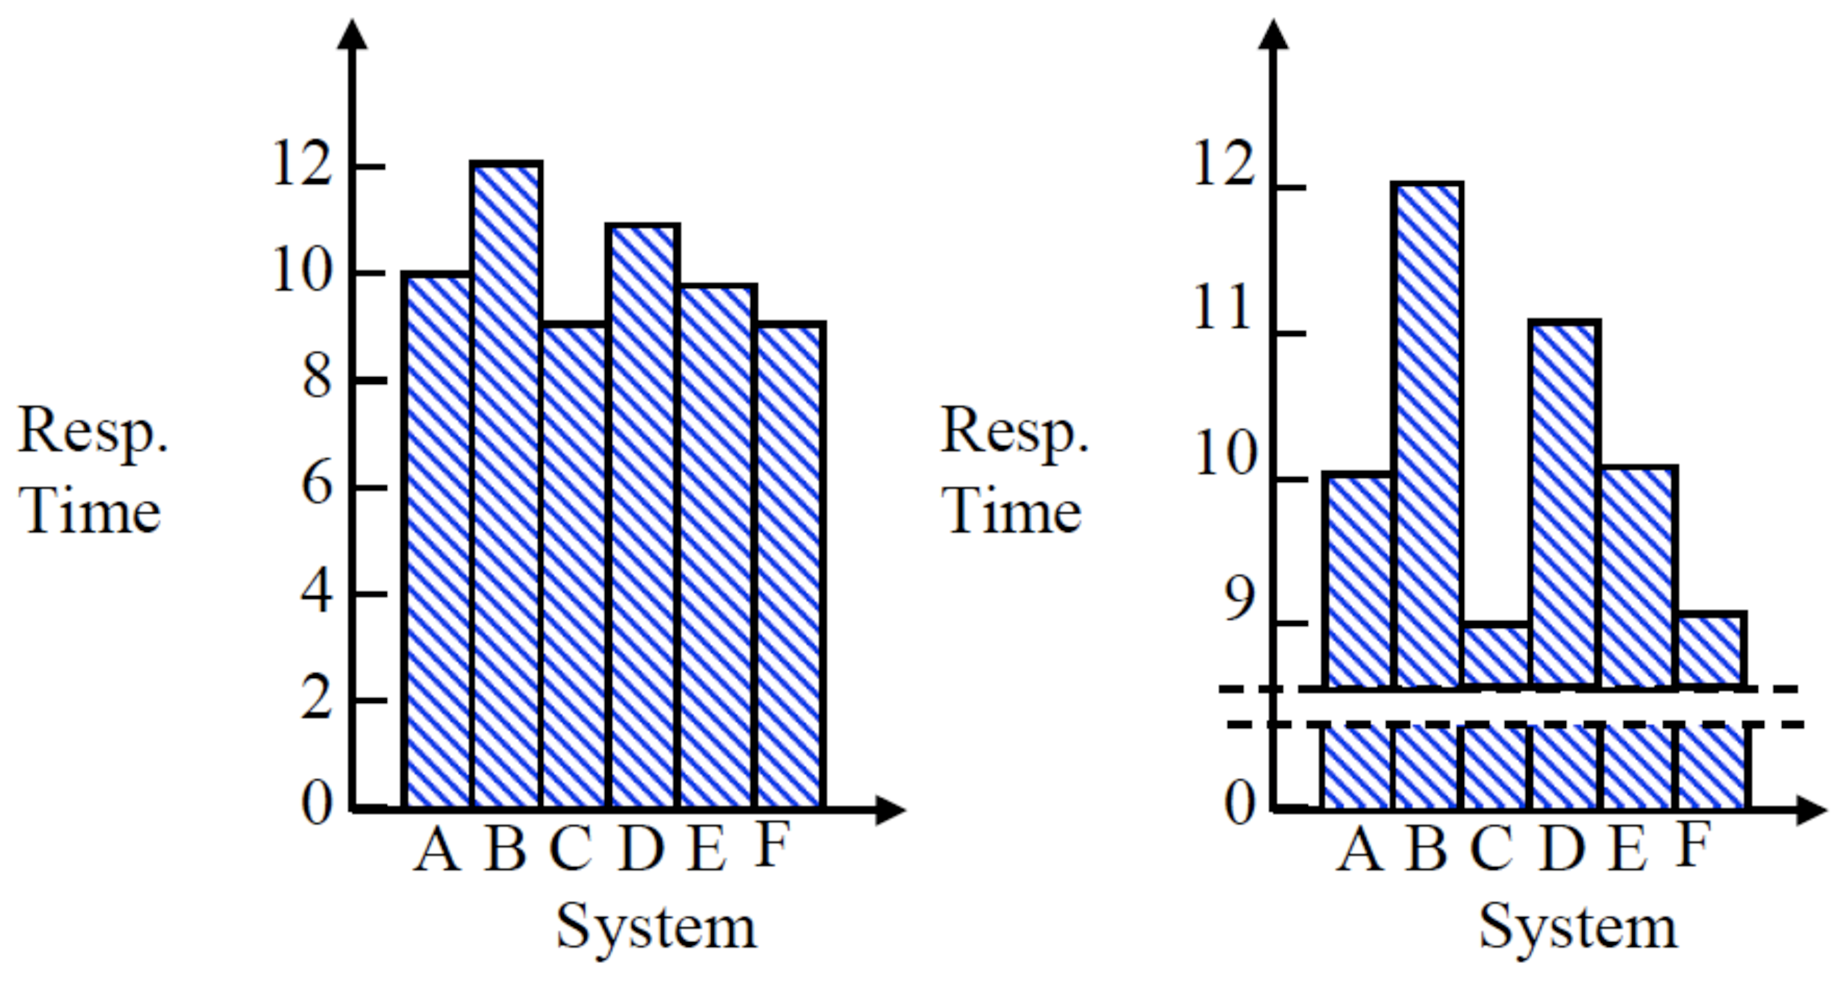
\includegraphics[width=10.8cm]{Jain-graph9}
\end{block}
\end{frame}

\section[{\scshape Principes}]{{\scshape Principes :} indicateurs}

\begin{frame}{Données}
\begin{alertblock}{Compréhension des données visualisées}
\begin{itemize}
\item  Le type de graphique est adapté aux données (courbe, bâtons, histogramme, nuages,...);
\item  Les interpolations/approximations ont un sens;
\item  Les courbes sont définies avec suffisamment de points;
\item  La méthode de construction de la courbe est claire: interpolation (linéaire, polynomiale,...), 
approximation (polynomiale, régression,...)
\item  Les intervalles de confiance sont visualisés (ou donnés séparément);
\item  Le pas de l'histogramme est adapté;
\item  L'ordonnée de l'histogramme est la probabilité (de $0$ à $1$).
\end{itemize}
\end{alertblock}
\end{frame}

\begin{frame}
\frametitle{Objets graphiques}
\begin{alertblock}{Éléments graphiques}
\begin{itemize}
\item  Les objets graphiques sont lisibles sur écran, impression couleur/noir et blanc, vidéo...
\item  La palette de couleur est standard, sans couleurs proches, sans vert (video); 
\item  Les axes du graphique sont bien identifiés et annotés; 
\item  Les échelles et les unités sont marquées; 
\item  Les courbes se croisent sans ambiguïté, en un point repérable; 
\item  Les grilles aident à lire la courbe.
\end{itemize}
\end{alertblock}
\end{frame}
\begin{frame}
\frametitle{Annotations}
\begin{alertblock}{Annotations et commentaires }
\begin{itemize}
\item  Les axes sont bien annotés par les quantités; 
\item  Le nom des axes est clair, concis et suffisamment explicatif;
\item  Les unités sont indiquées sur les axes;
\item  Les axes sont orientés du plus petit au plus grand de gauche à droite et de bas en haut;
\item  L'origine est $(0,0)$ sinon c'est justifié;
\item  Les échelles sont contigües.
\item  Pour les diagrammes en bâton/histogrammes l'ordre des bâtons est systématique (alphabétique, temporel, du meilleur au moins bon sont préférables à un ordre aléatoire)
\item  Les courbes sont annotées individuellement (légende); 
\item  Les barres/rectangles sont annotés individuellement (légende).
\end{itemize}
\end{alertblock}
\end{frame}

\begin{frame}
\frametitle{Message}
\begin{alertblock}{Information : ce que dit le graphique}
\begin{itemize}
\item  Les courbes sont mises sur la même échelle;
\item  Le nombre de courbes est petit (pas plus de $6$);
\item  Les courbes à comparer sont sur le même graphique;
\item  On ne peut pas supprimer une courbe sans diminuer significativement l'information donnée par le graphique;
\item  Le graphique fournit une information pertinente au lecteur;
\item  Si l'axe vertical représente une quantité aléatoire, il présente des barres d'erreur;
\item  Peut-on supprimer des objets graphiques, du texte, des courbes \\
sans modifier la compréhension ?
\end{itemize}
\end{alertblock}
\end{frame}

\begin{frame}
\frametitle{Contexte}

\begin{alertblock}{Contexte du graphique}
\begin{itemize}
\item  Tous les symboles du graphique sont référencés (définis) dans le texte;
\item  Les variables tracées fournissent plus d'informations que des représentations alternatives; (choix d'autres variables)
\item  Le graphique a un titre;
\item  Le titre est autosuffisant pour comprendre partiellement le graphique;
\item  La figure est référencée dans le corps du texte;
\item  La figure est commentée dans le texte.
\end{itemize}
\end{alertblock}
\end{frame}
%{\large \textbf{Enfin}}: {\large \textbf{Le graphique doit être beau}}

\section[{\scshape Exemples}]{{\scshape Exemples :} illustration}
\begin{frame}{Example (1)}
\begin{center}
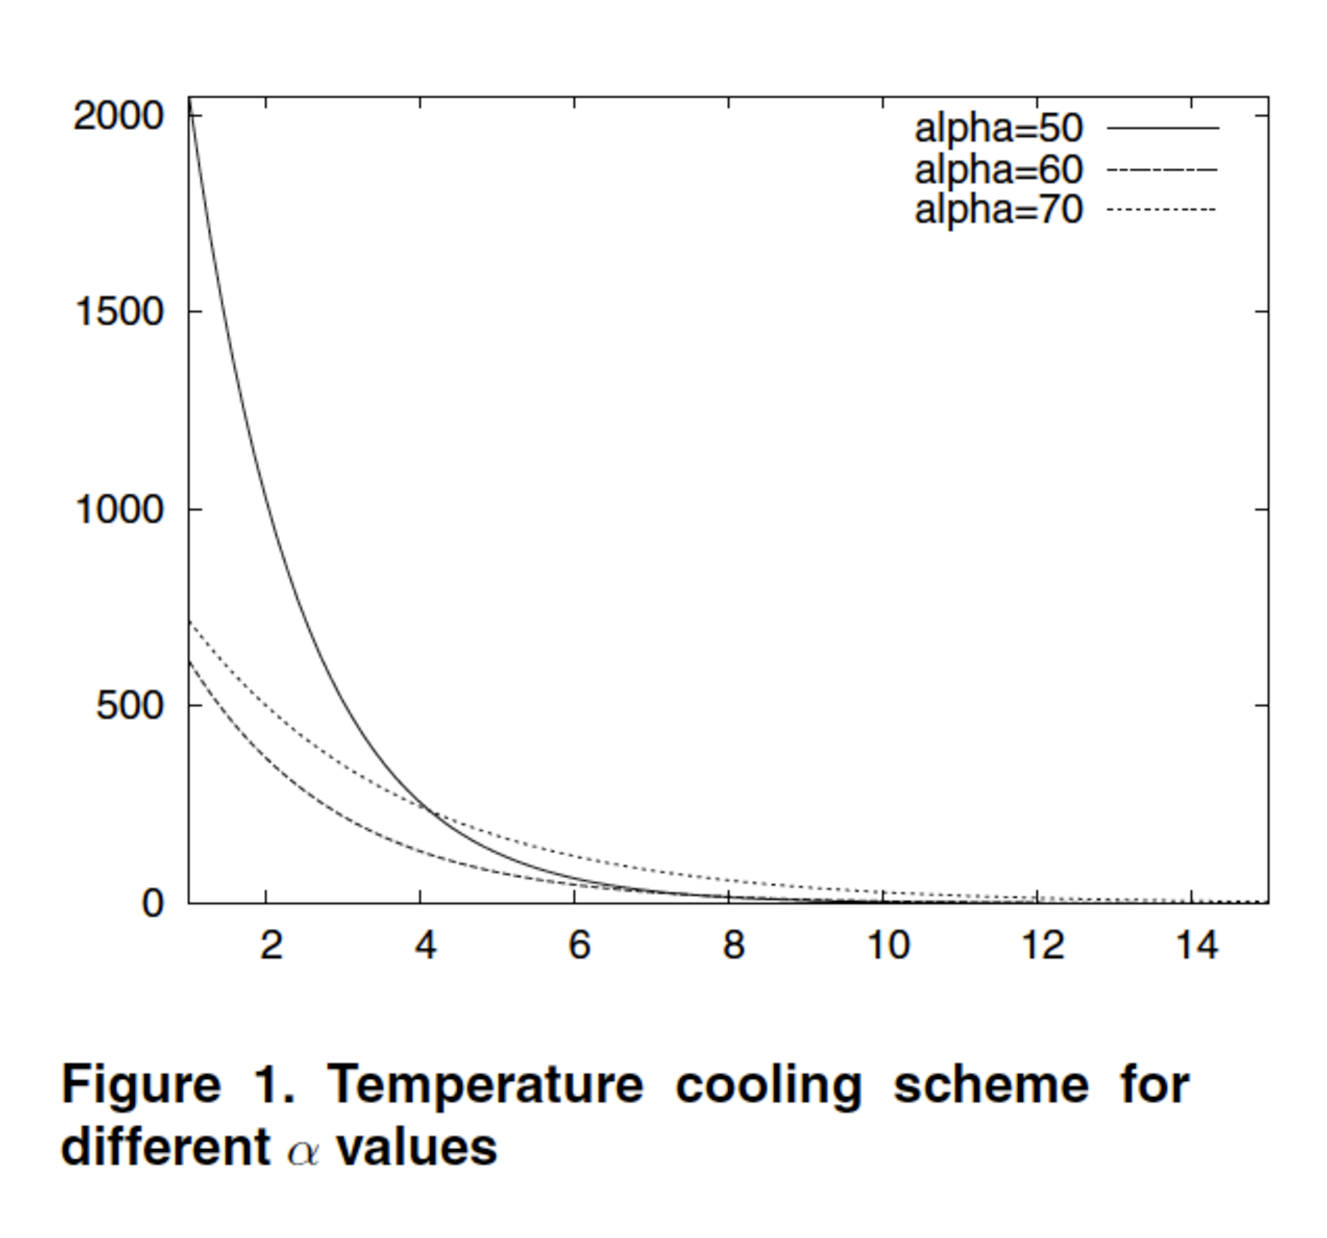
\includegraphics[width=0.8\textwidth]{Example1}
\end{center}
\end{frame}

\begin{frame}{Example (2)}
\begin{center}
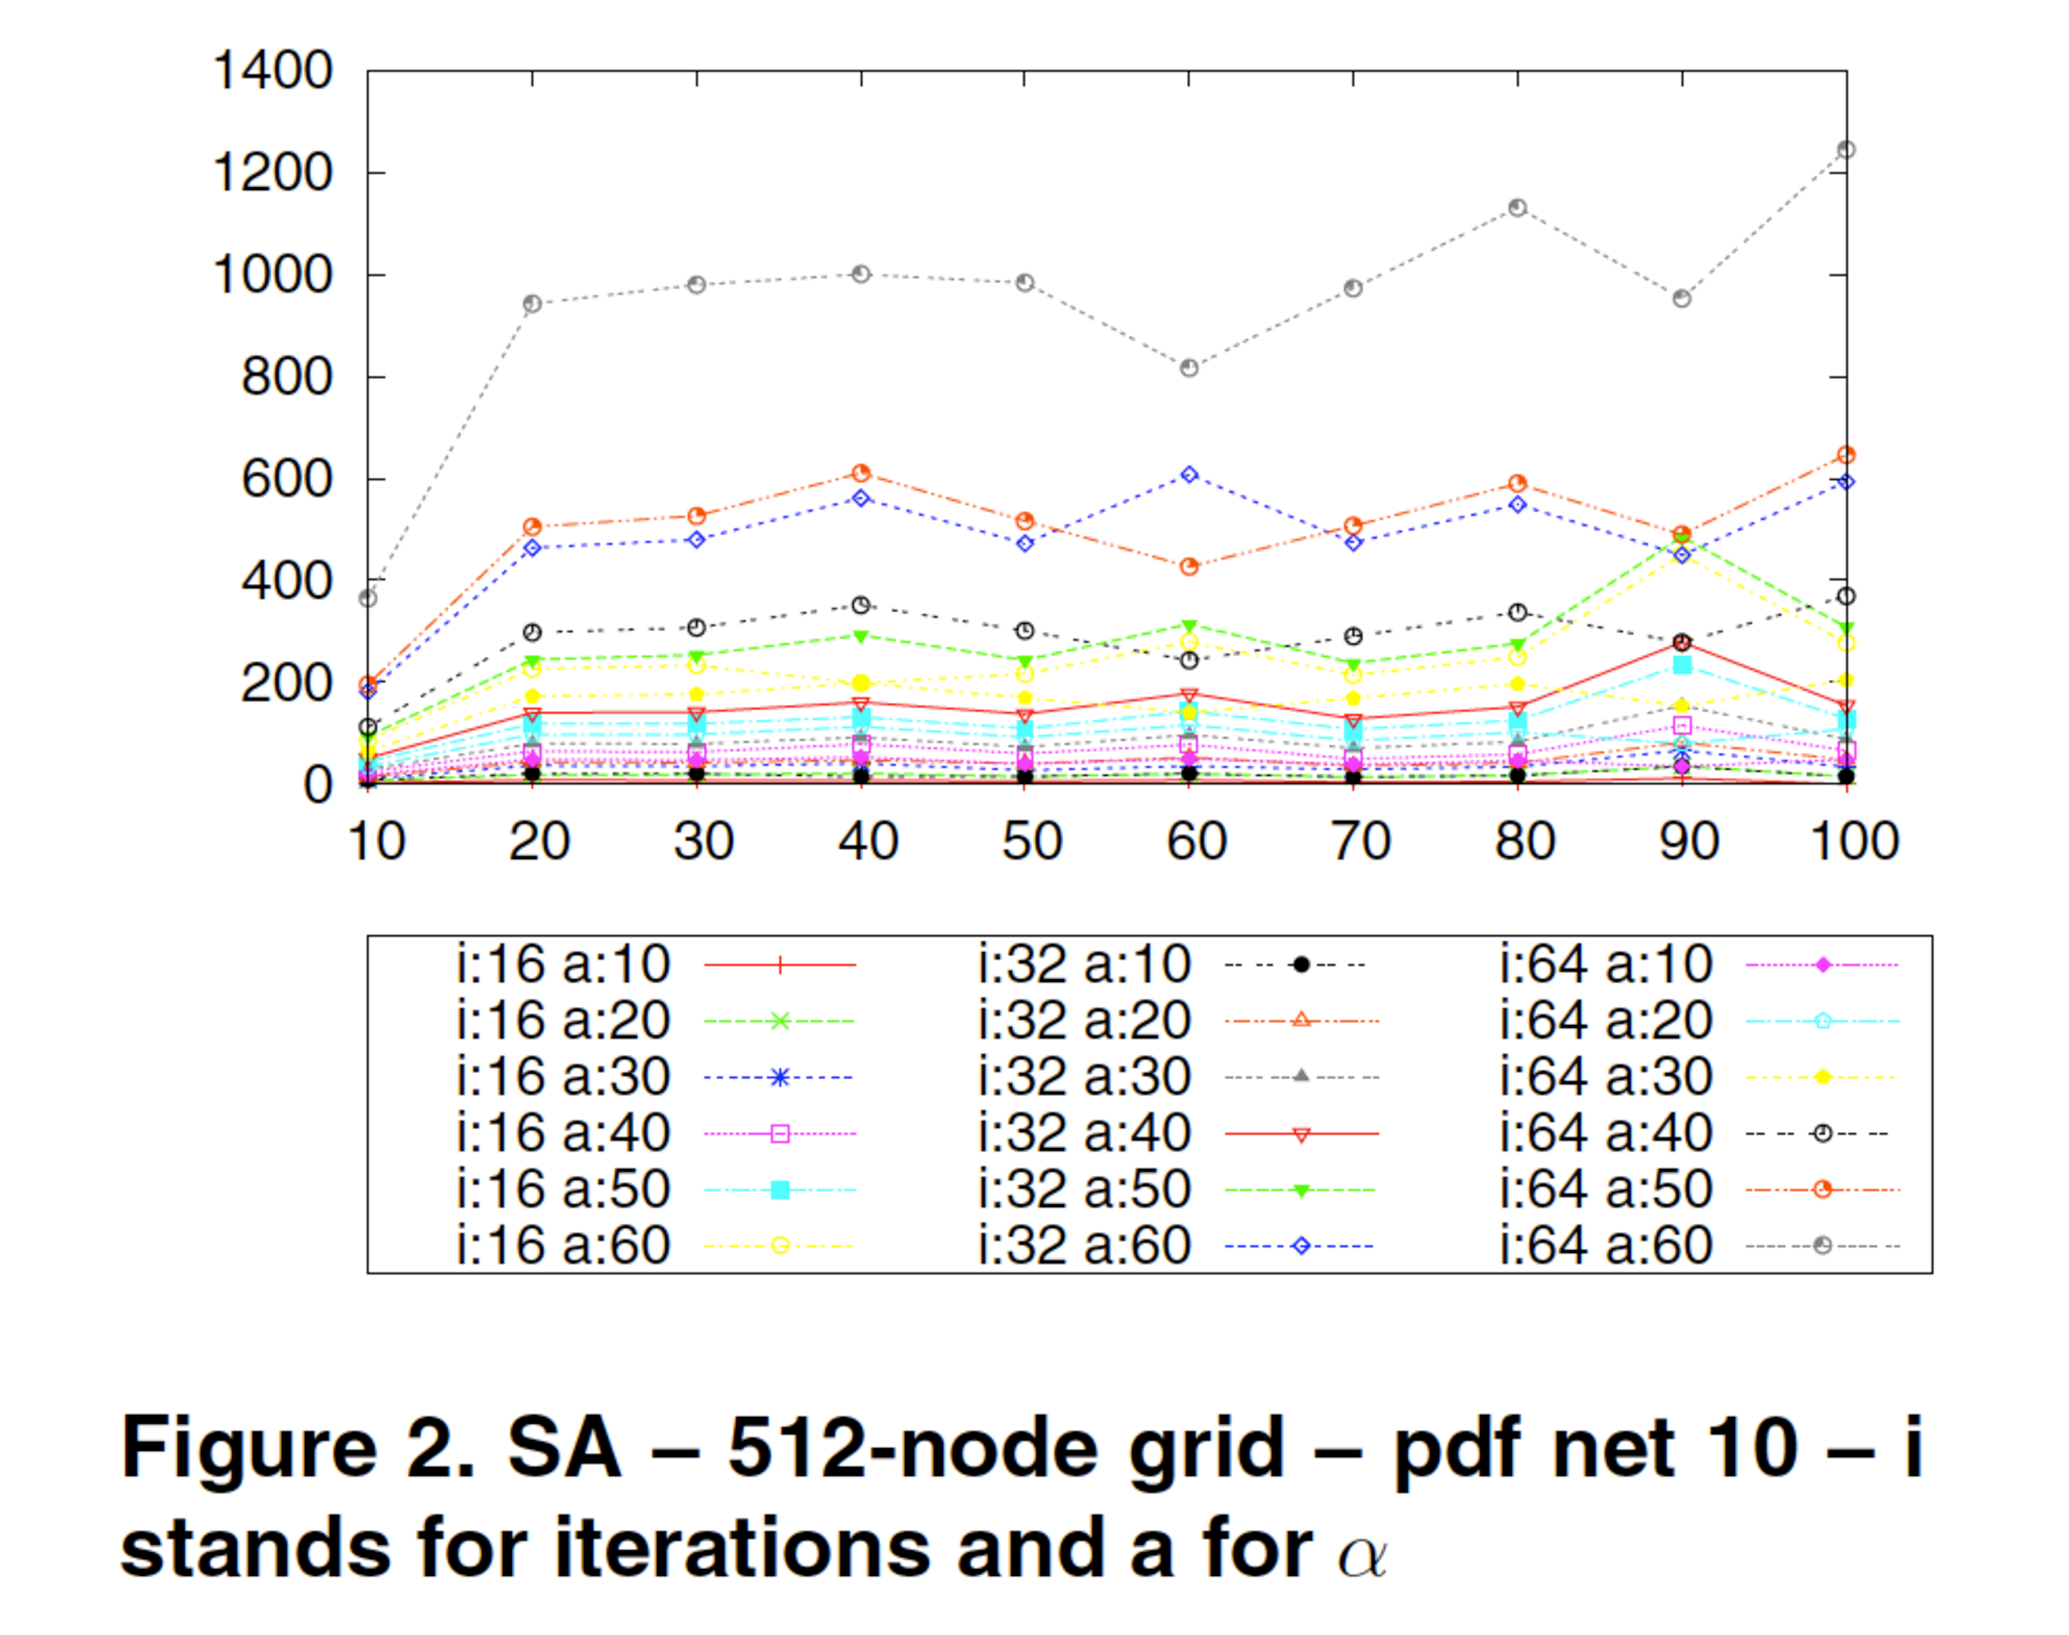
\includegraphics[width=0.8\textwidth]{Example2}
\end{center}
\end{frame}

\begin{frame}{Example (3)}
\begin{center}
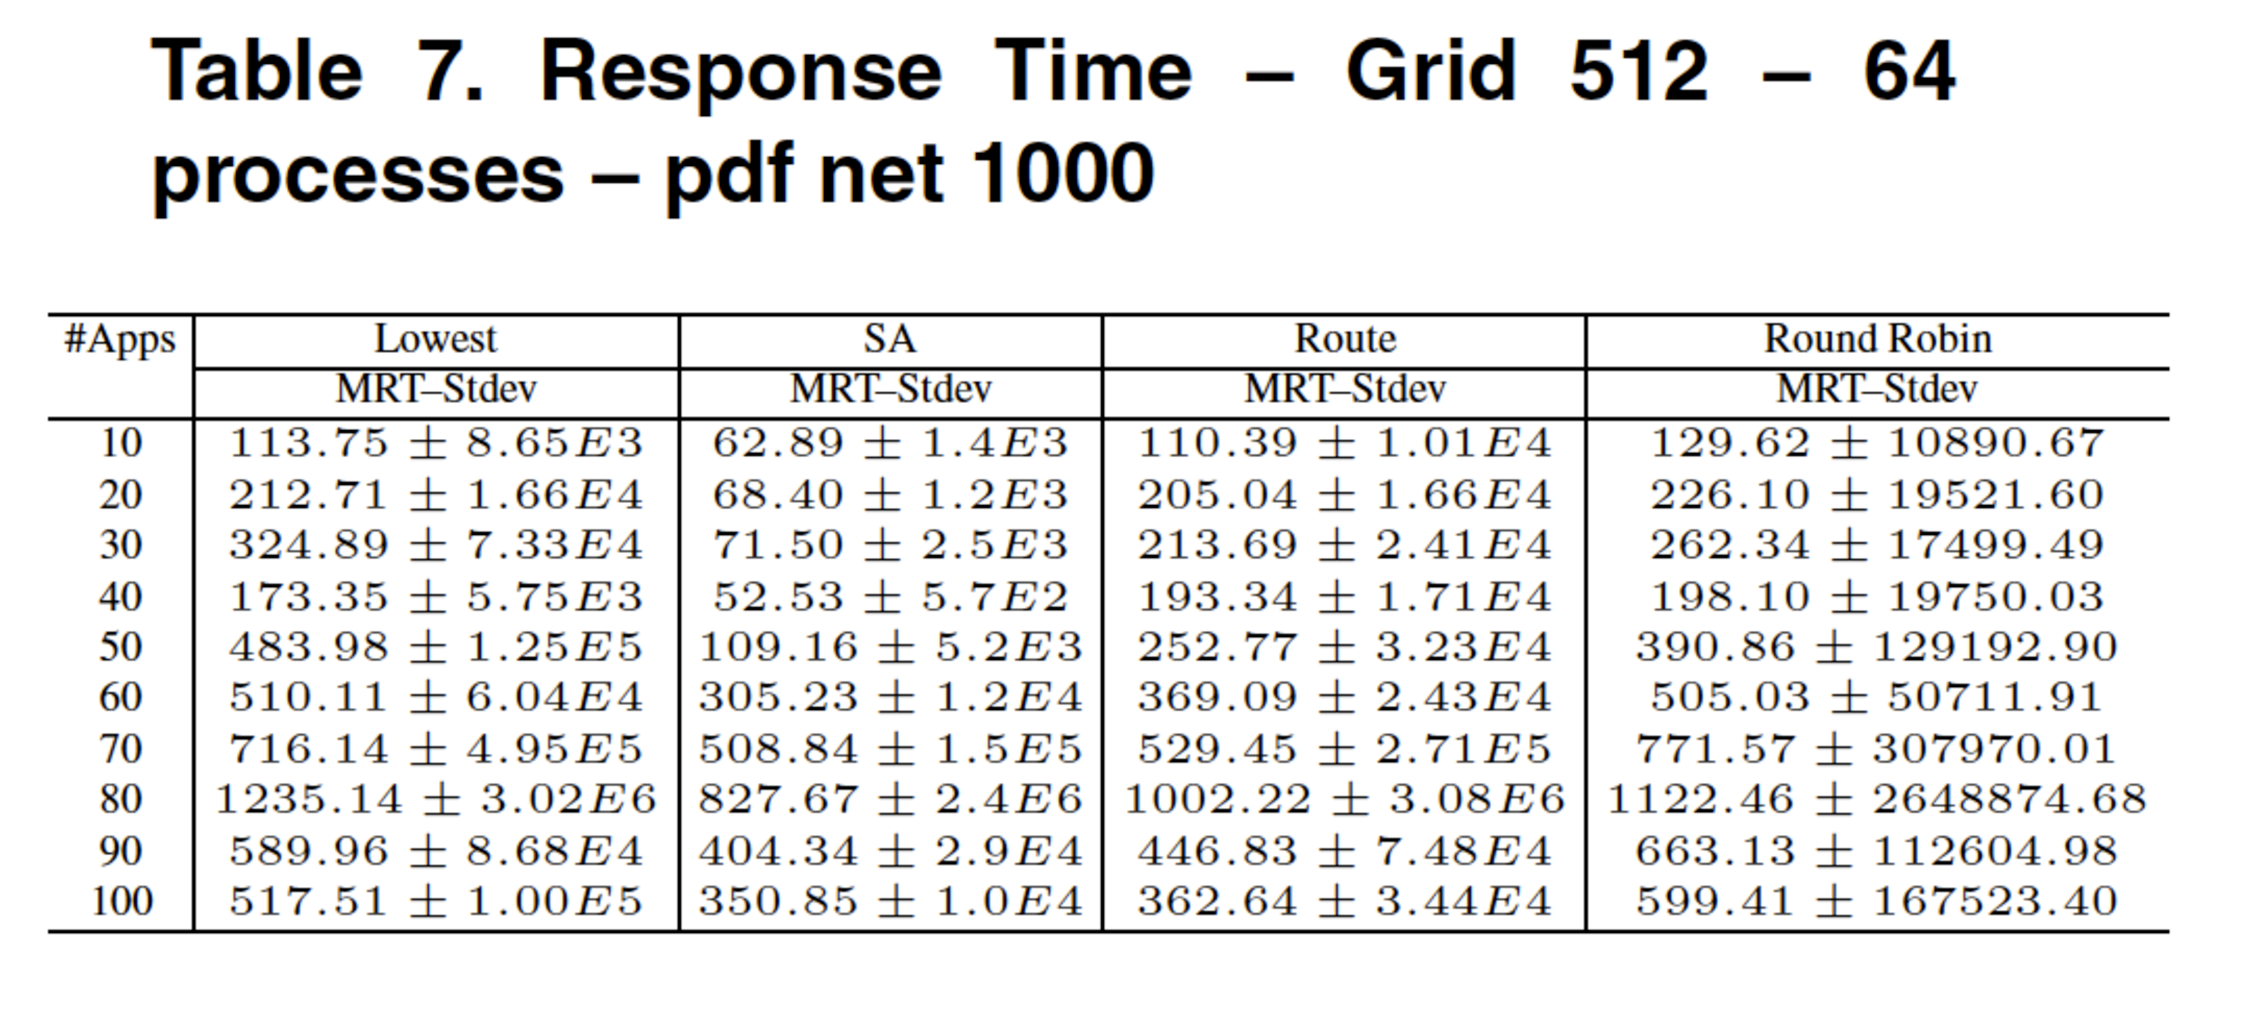
\includegraphics[width=0.8\textwidth]{Example3}
\end{center}
\end{frame}
\begin{frame}{Example (4)}
\begin{center}
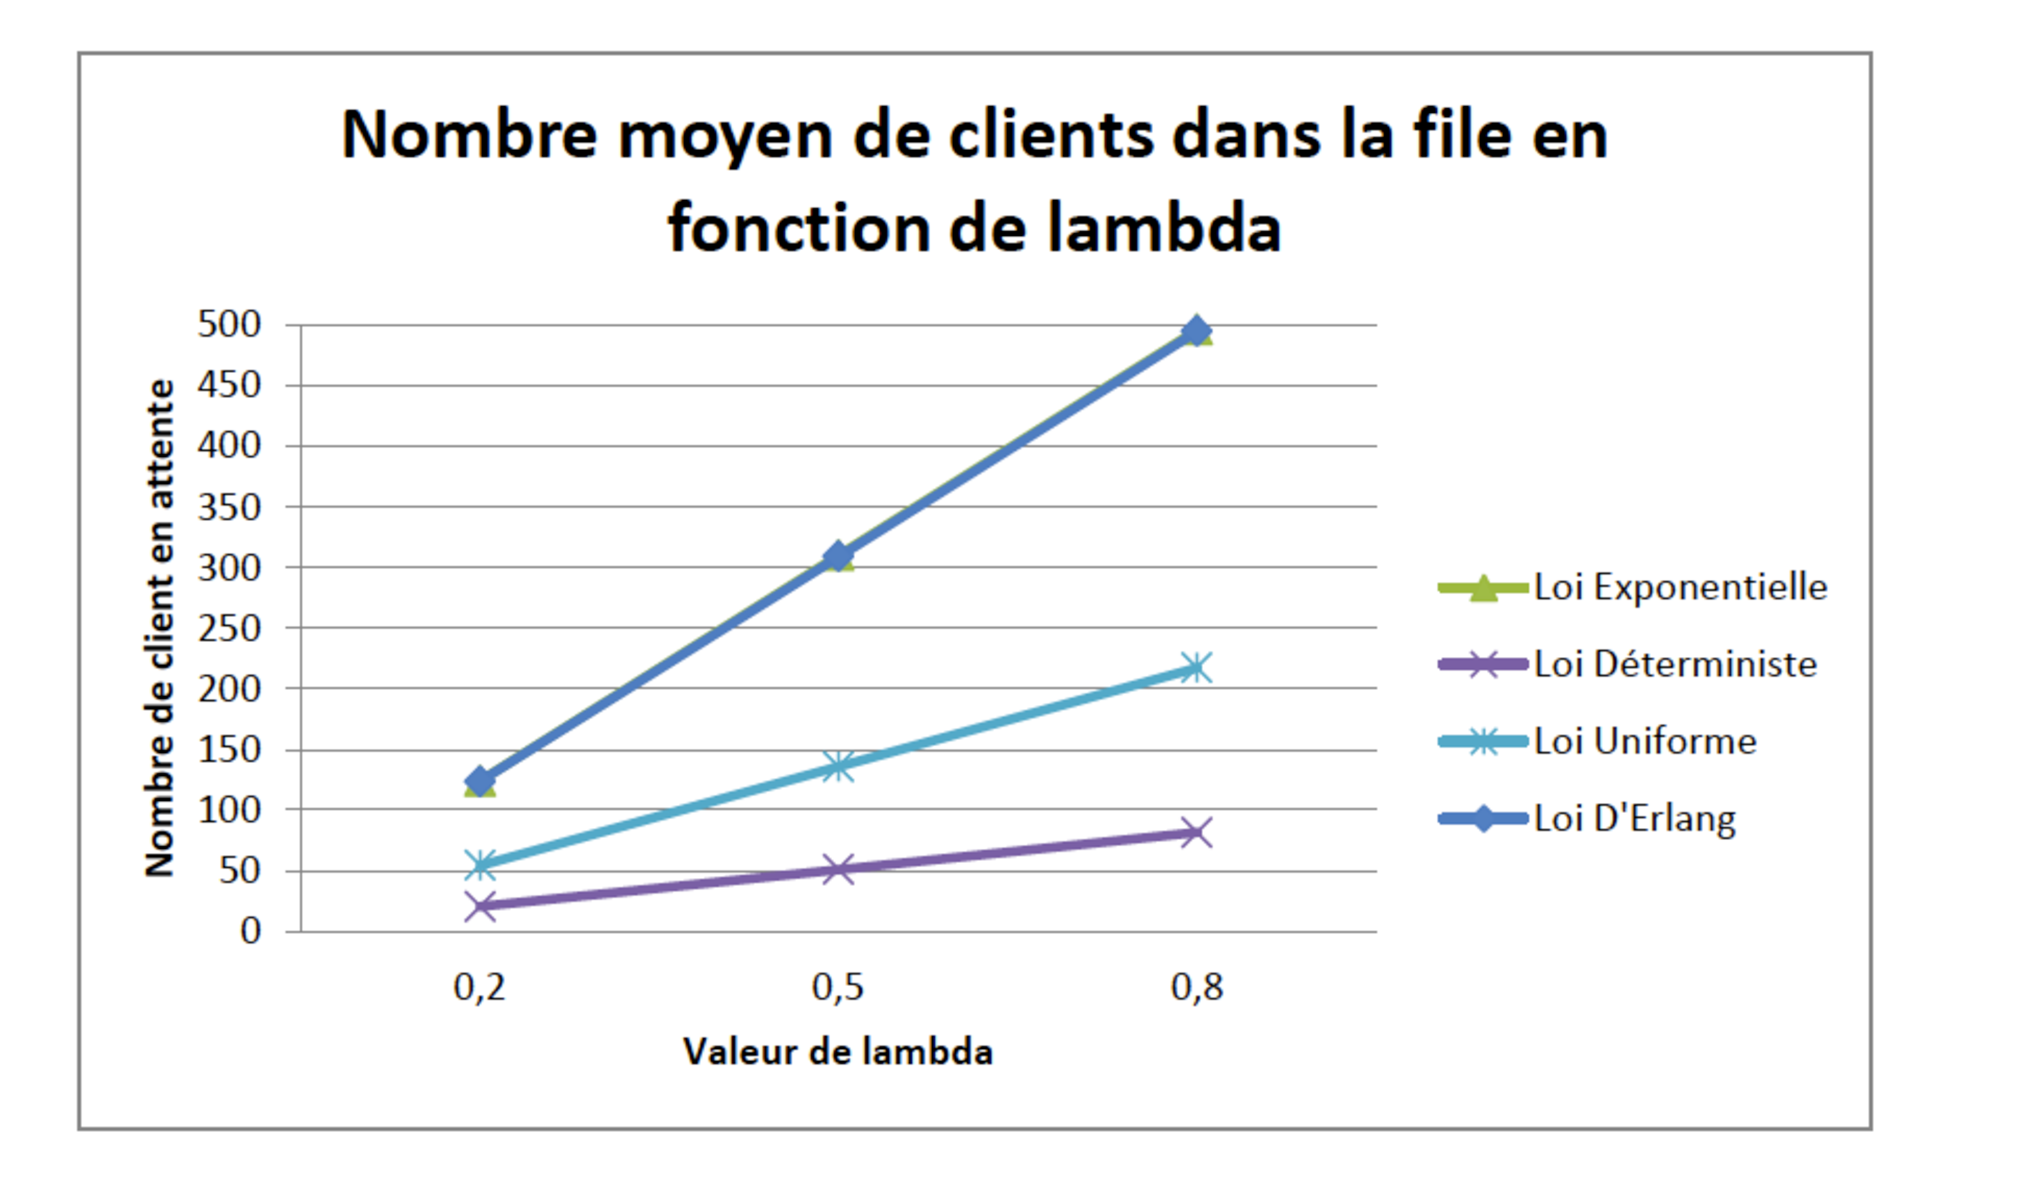
\includegraphics[width=0.8\textwidth]{Example4}
\end{center}
\end{frame}
\begin{frame}{Example (5)}
\begin{center}
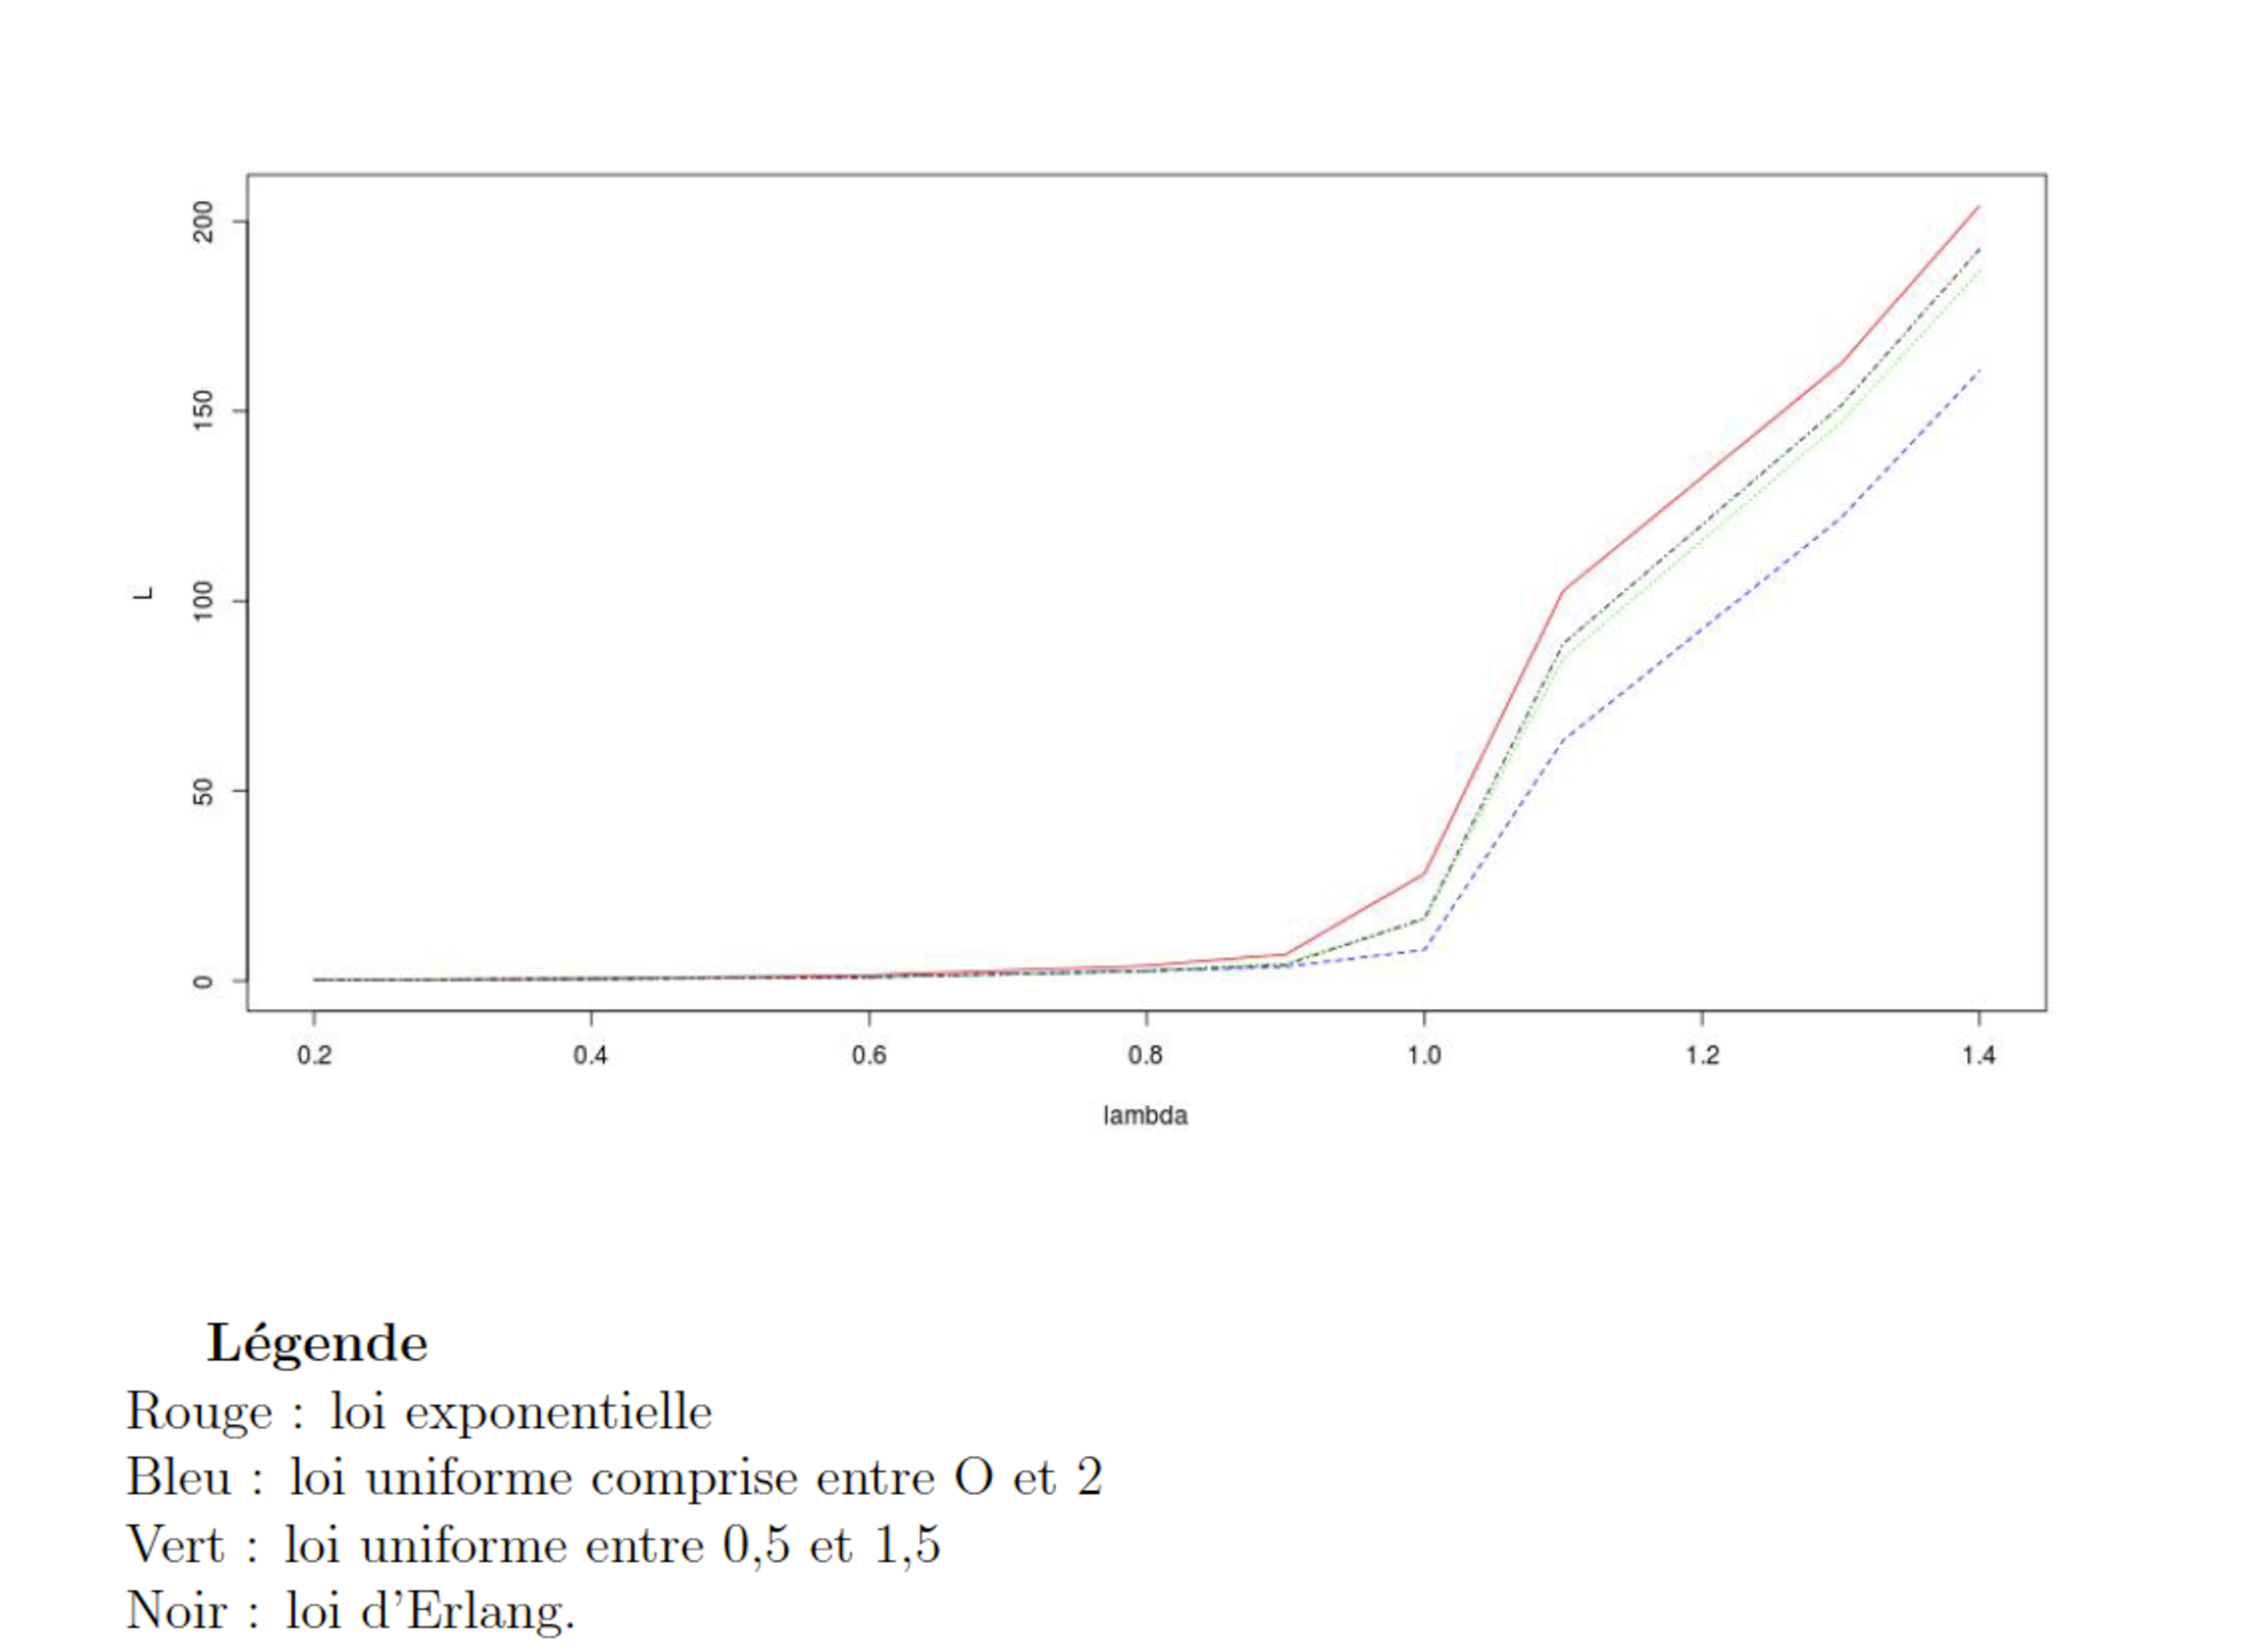
\includegraphics[width=0.8\textwidth]{Example5}
\end{center}
\end{frame}
\begin{frame}{Example (6)}
\begin{center}
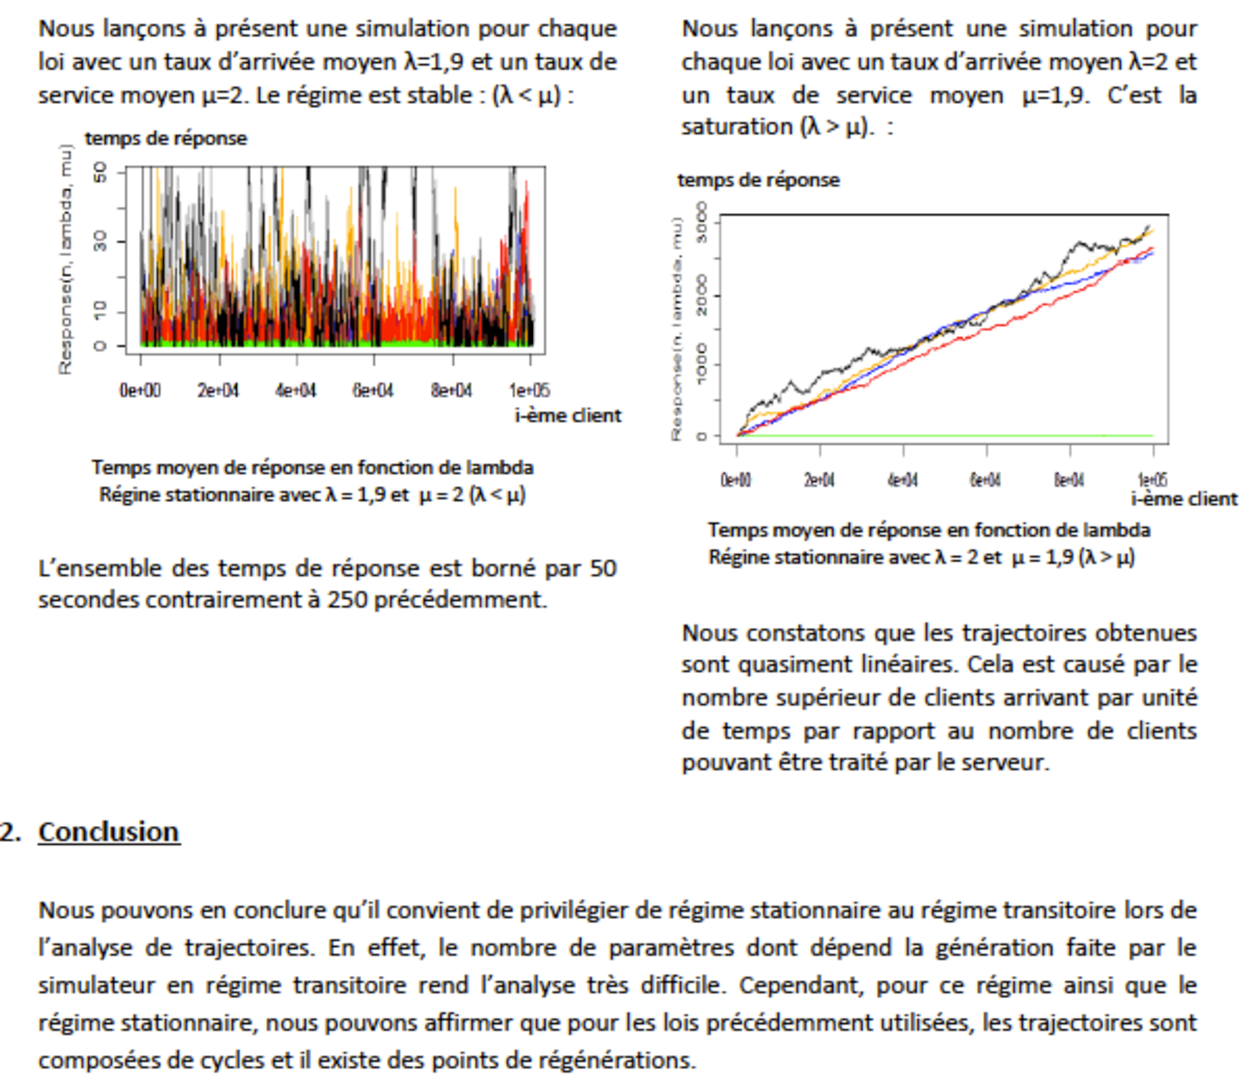
\includegraphics[width=0.8\textwidth]{Example6}
\end{center}
\end{frame}
\begin{frame}{Example (7)}
\begin{center}
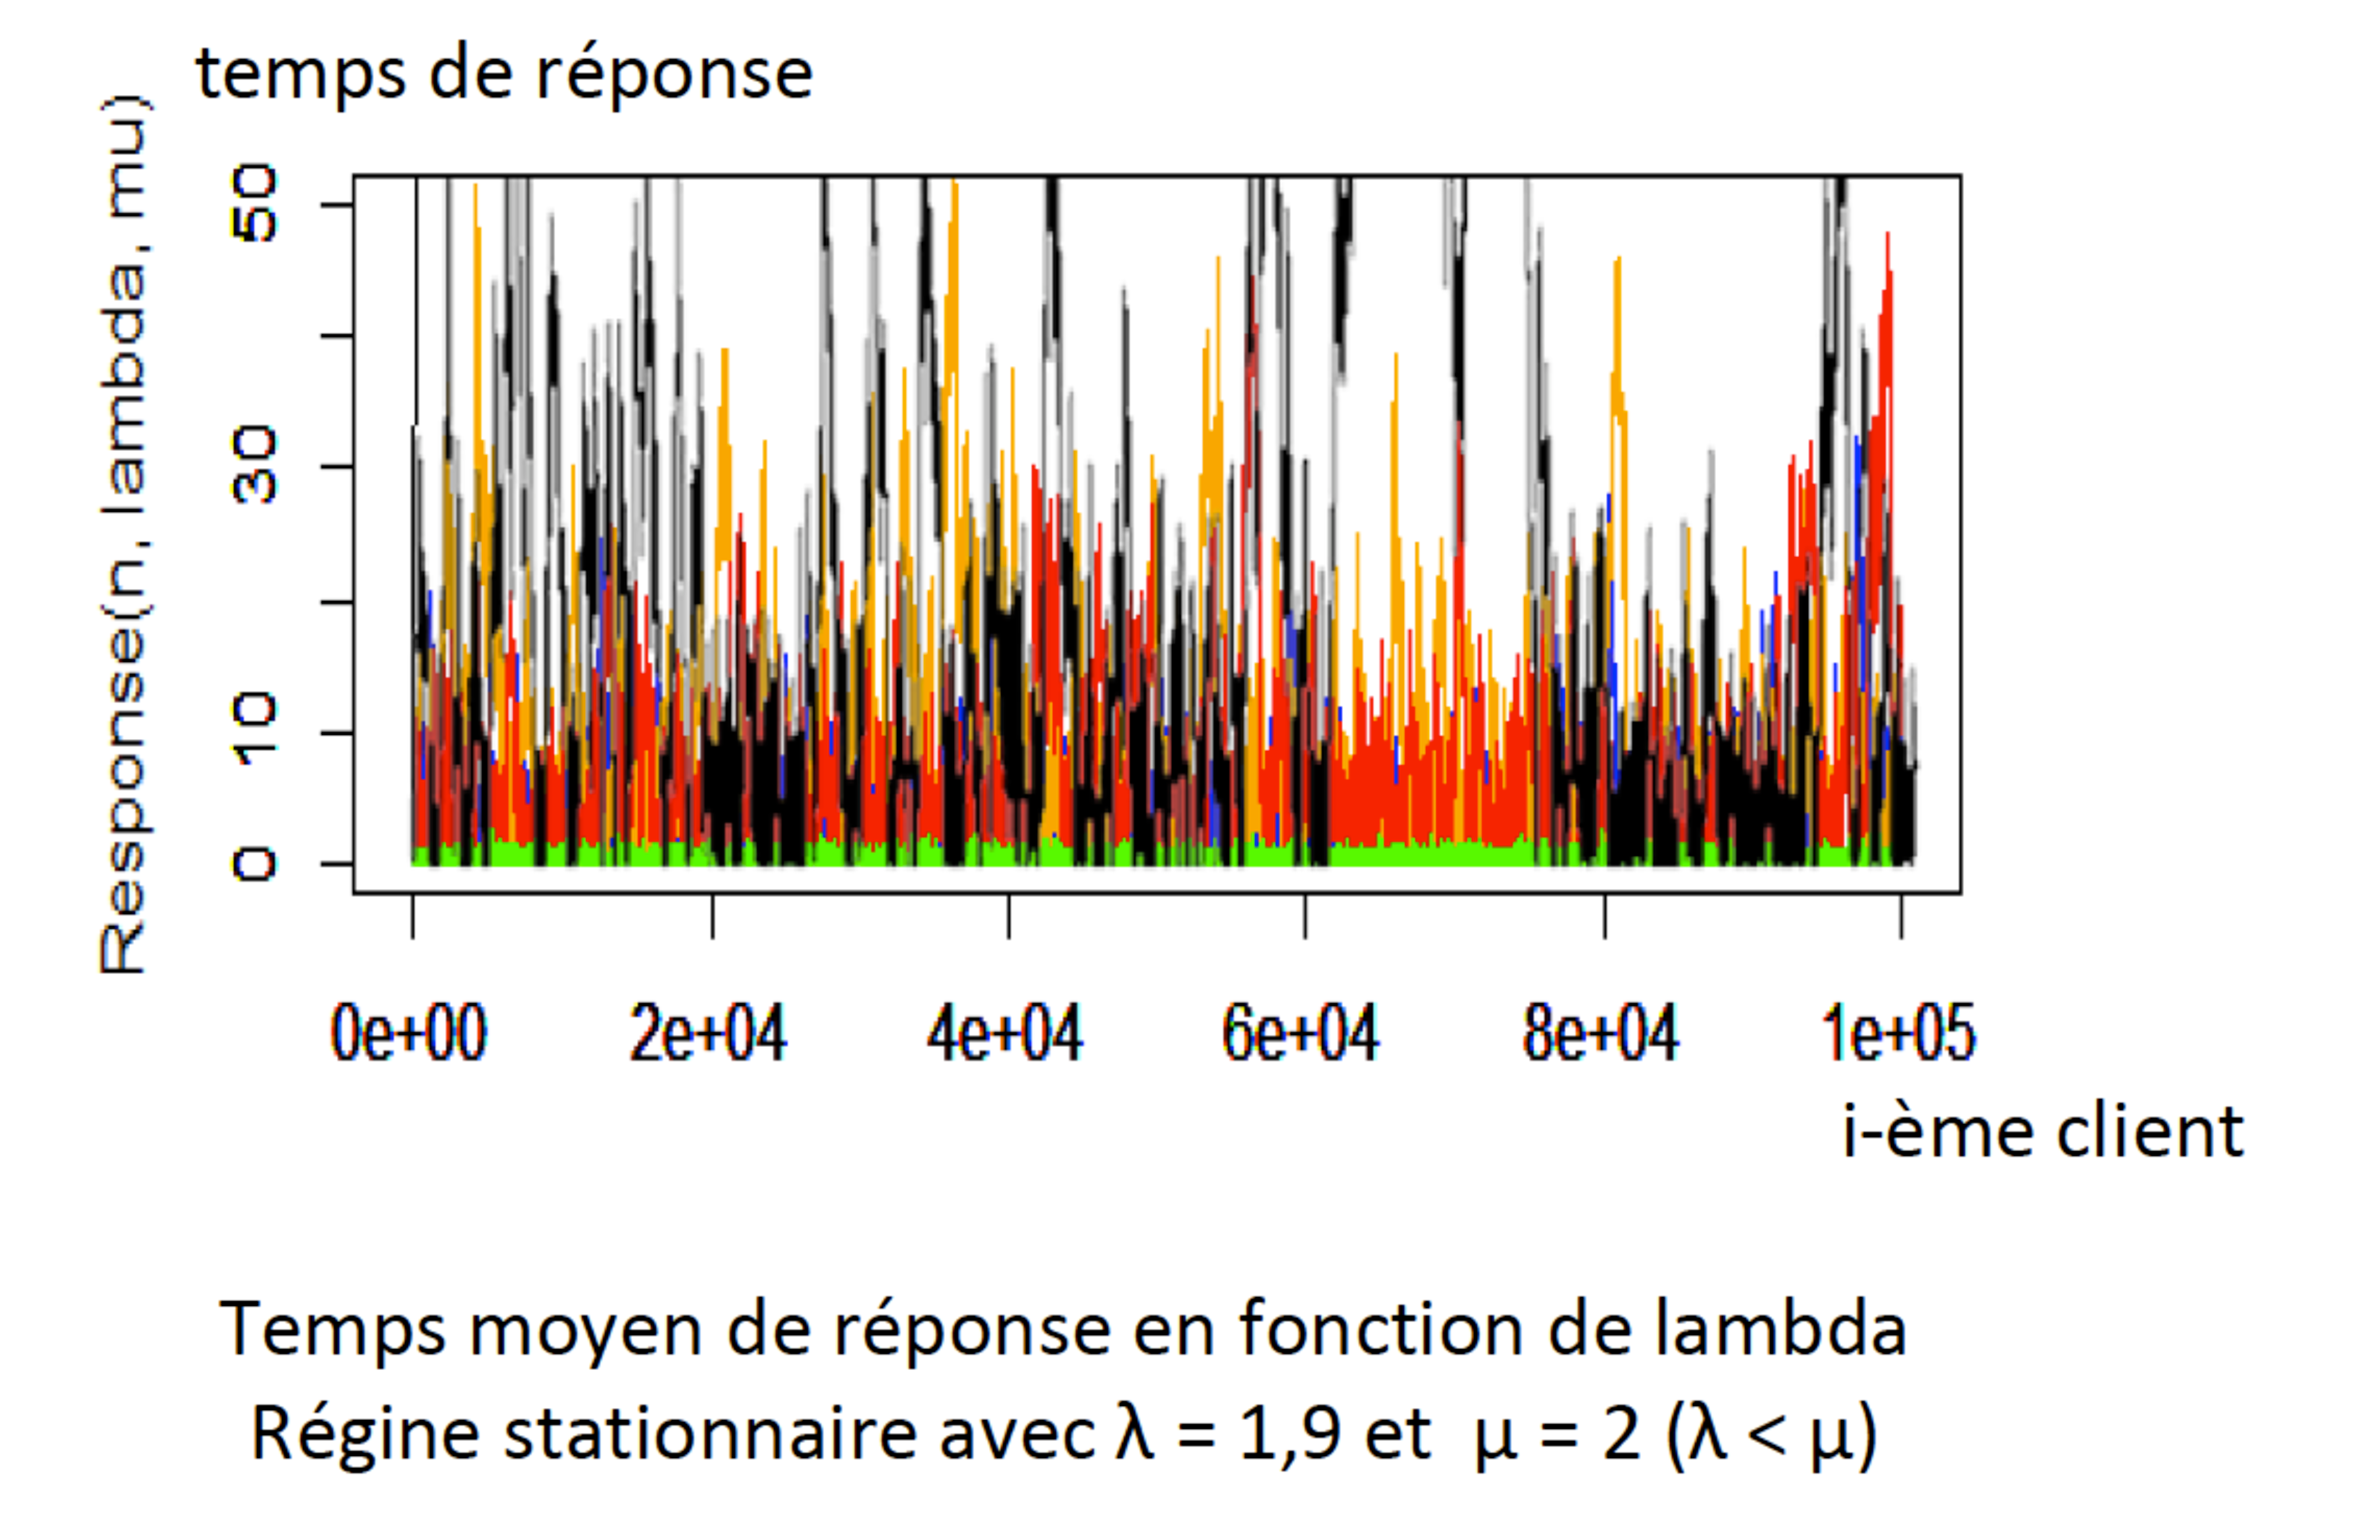
\includegraphics[width=0.8\textwidth]{Example7}
\end{center}
\end{frame}
\begin{frame}{Example (8)}
\begin{center}
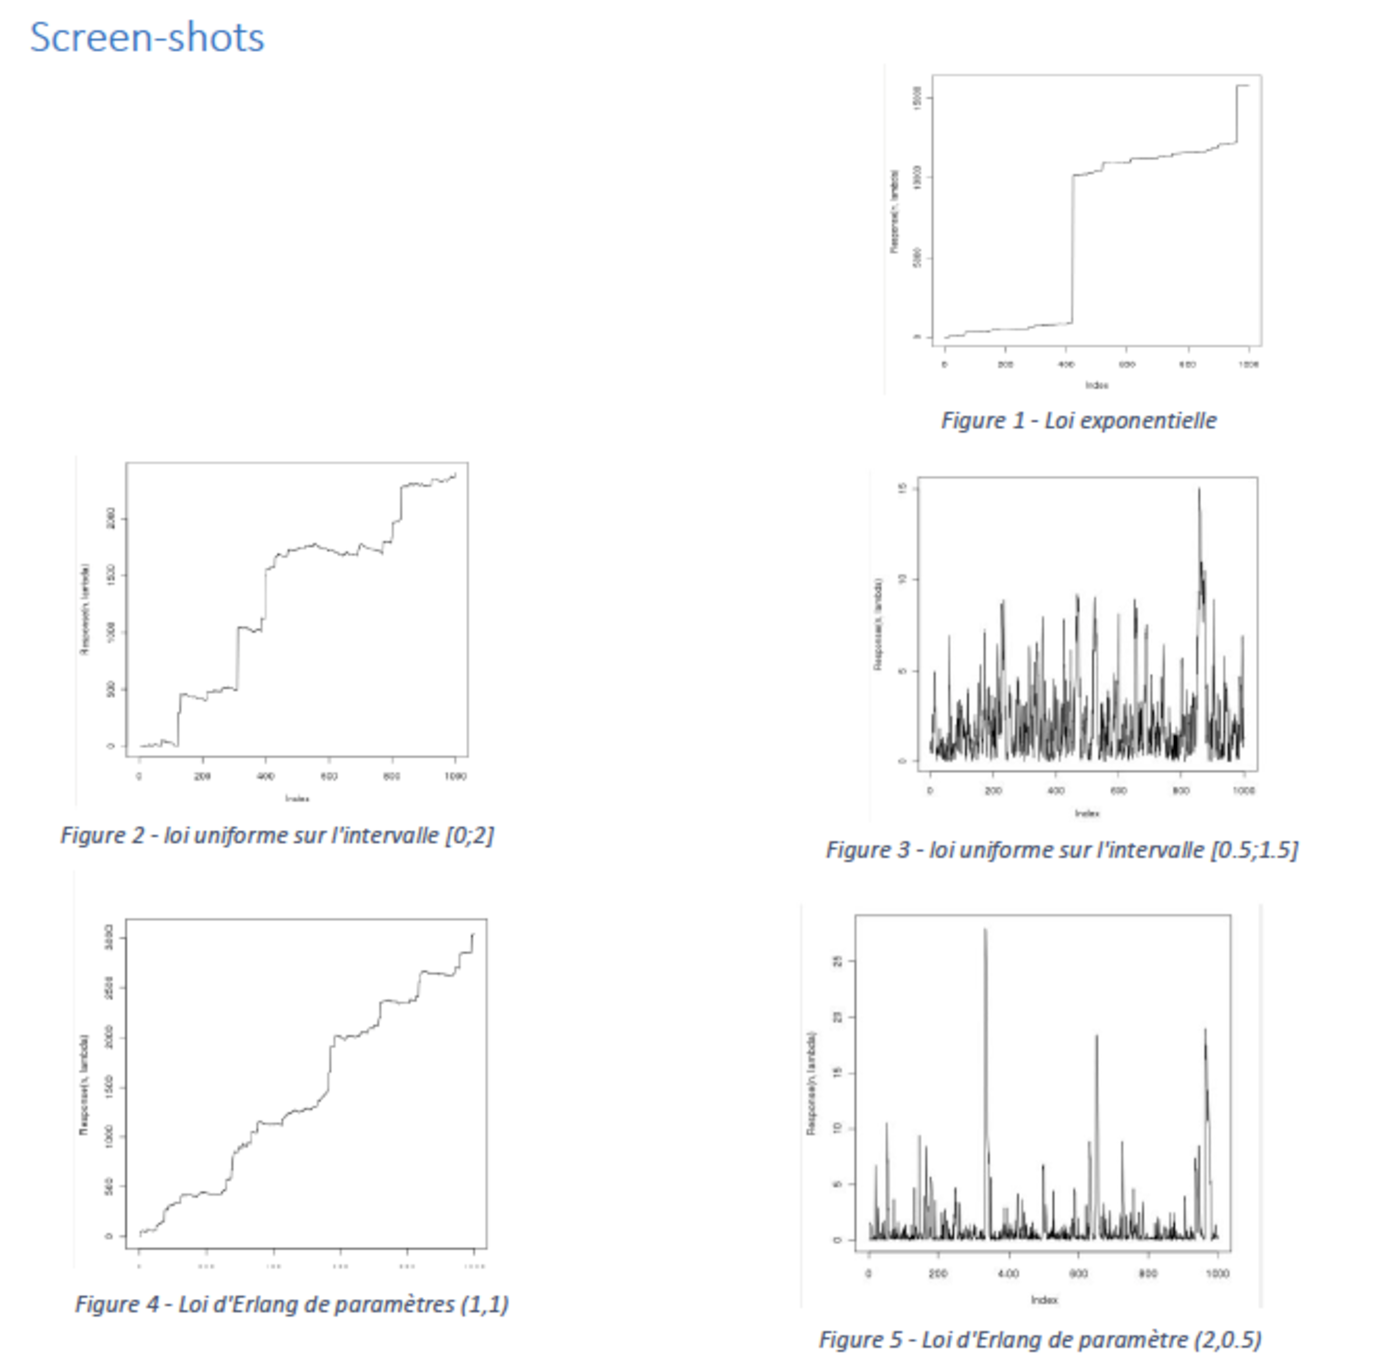
\includegraphics[width=0.8\textwidth]{Example8}
\end{center}
\end{frame}
\begin{frame}{Example (9)}
\begin{center}
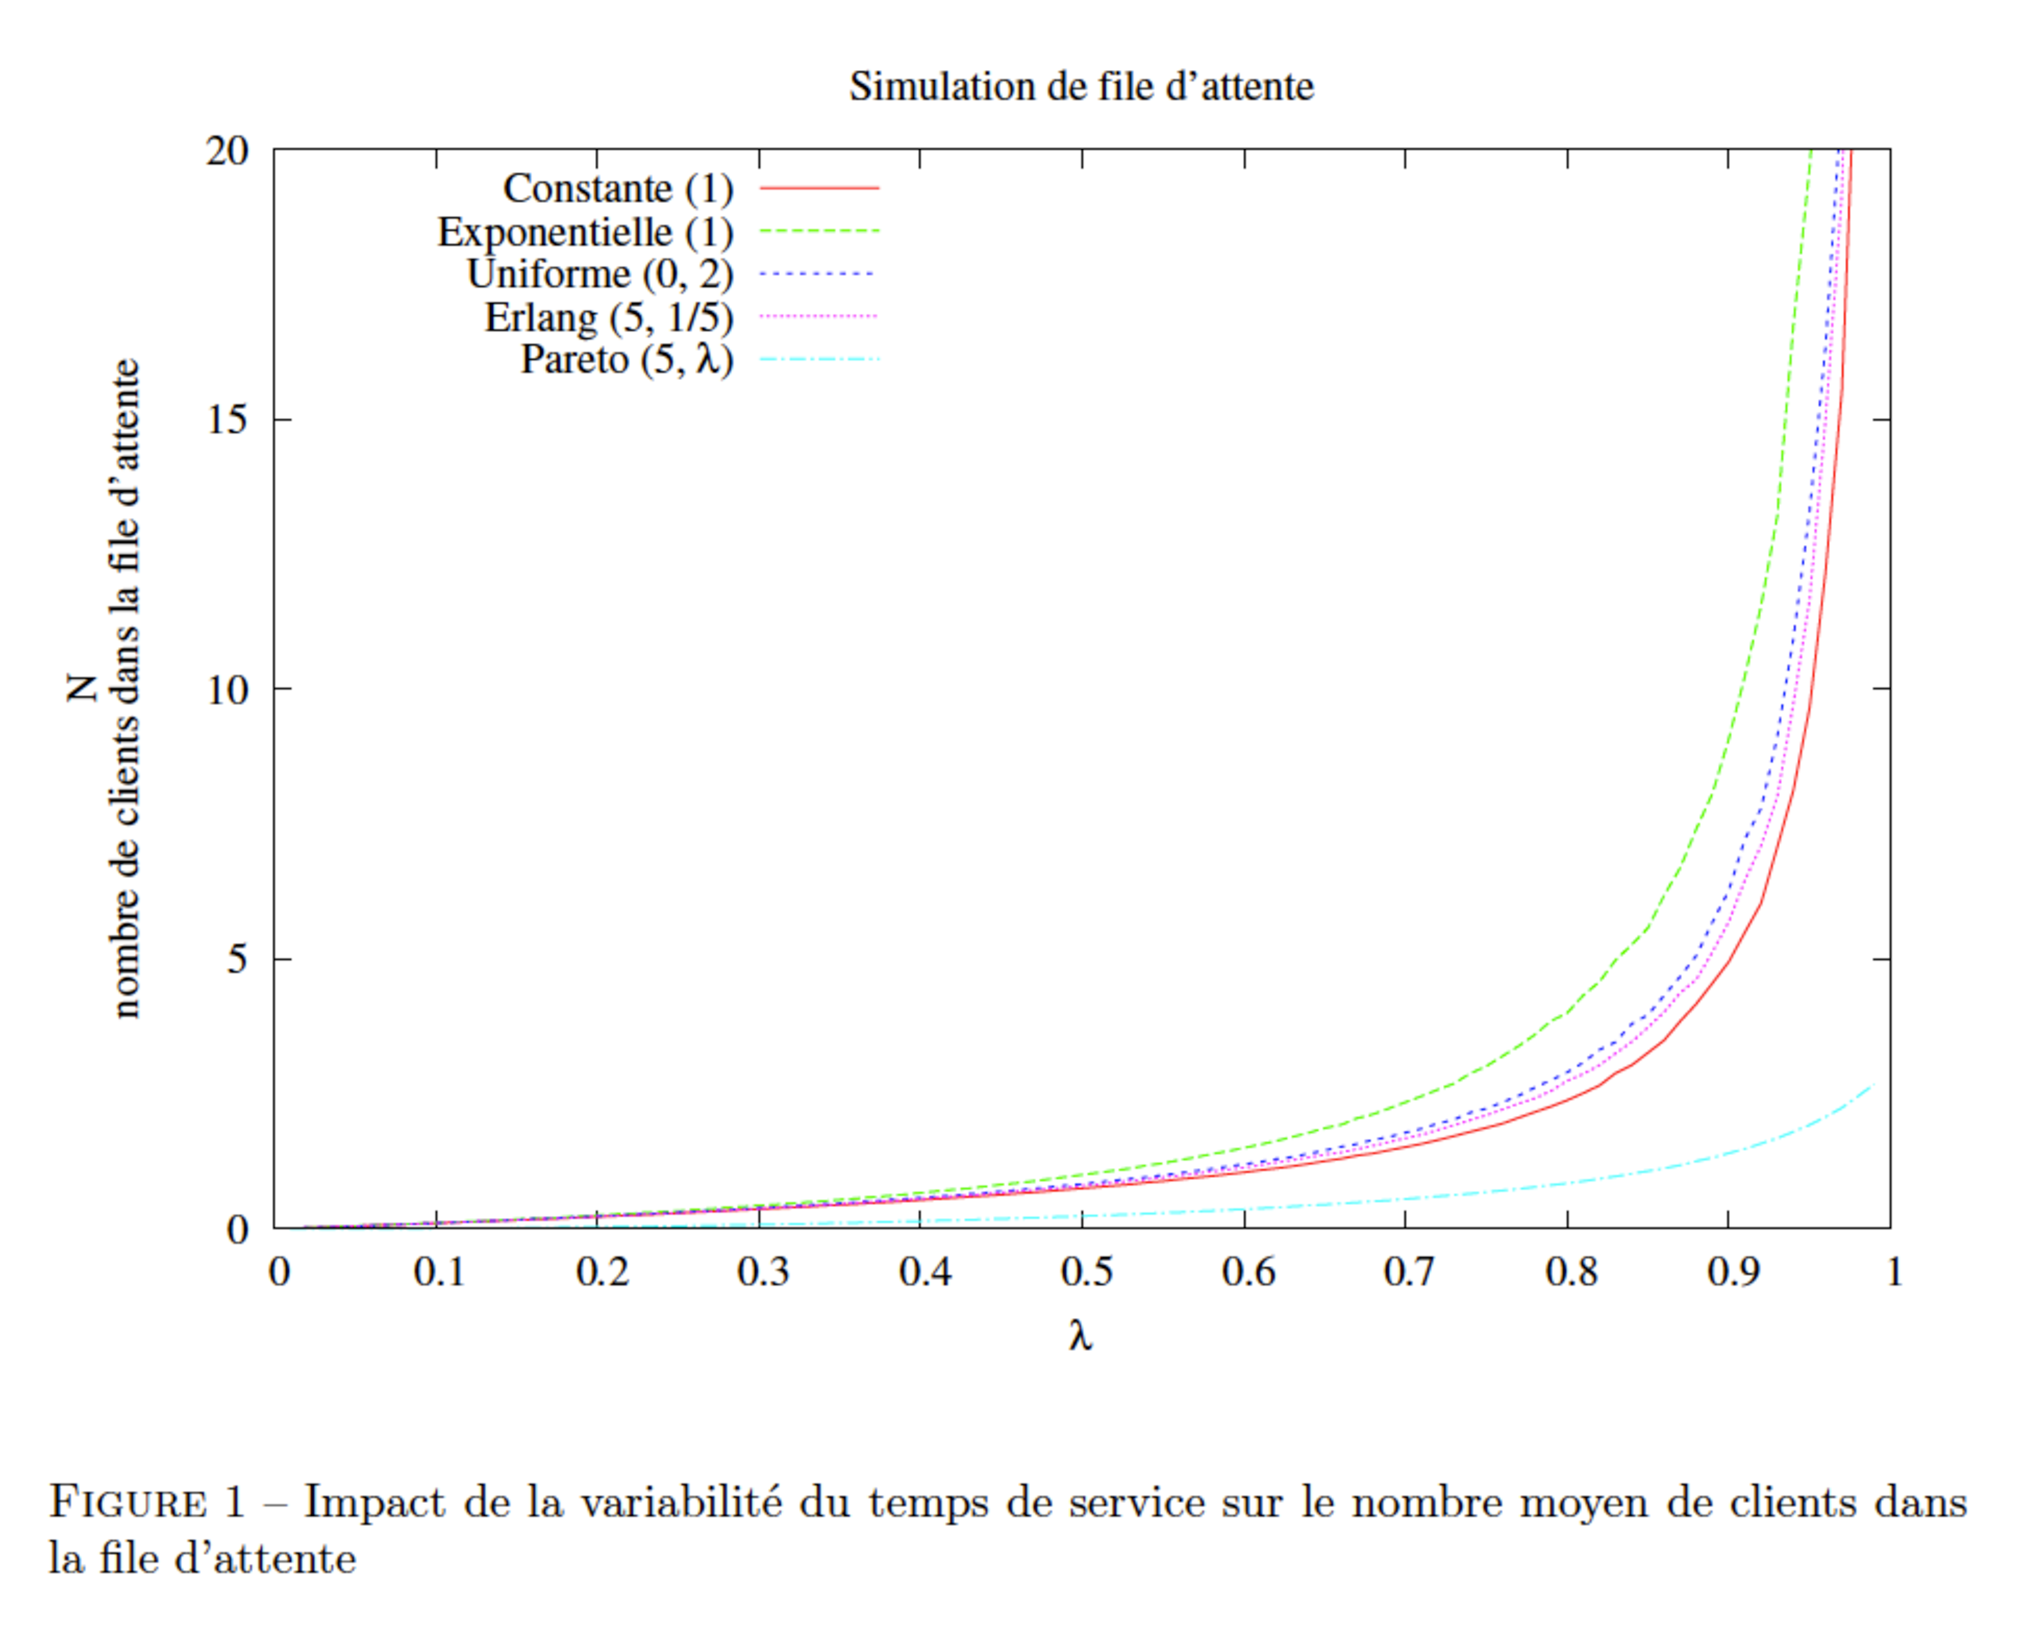
\includegraphics[width=0.8\textwidth]{Example9}
\end{center}
\end{frame}
\begin{frame}{Example (10)}
\begin{center}
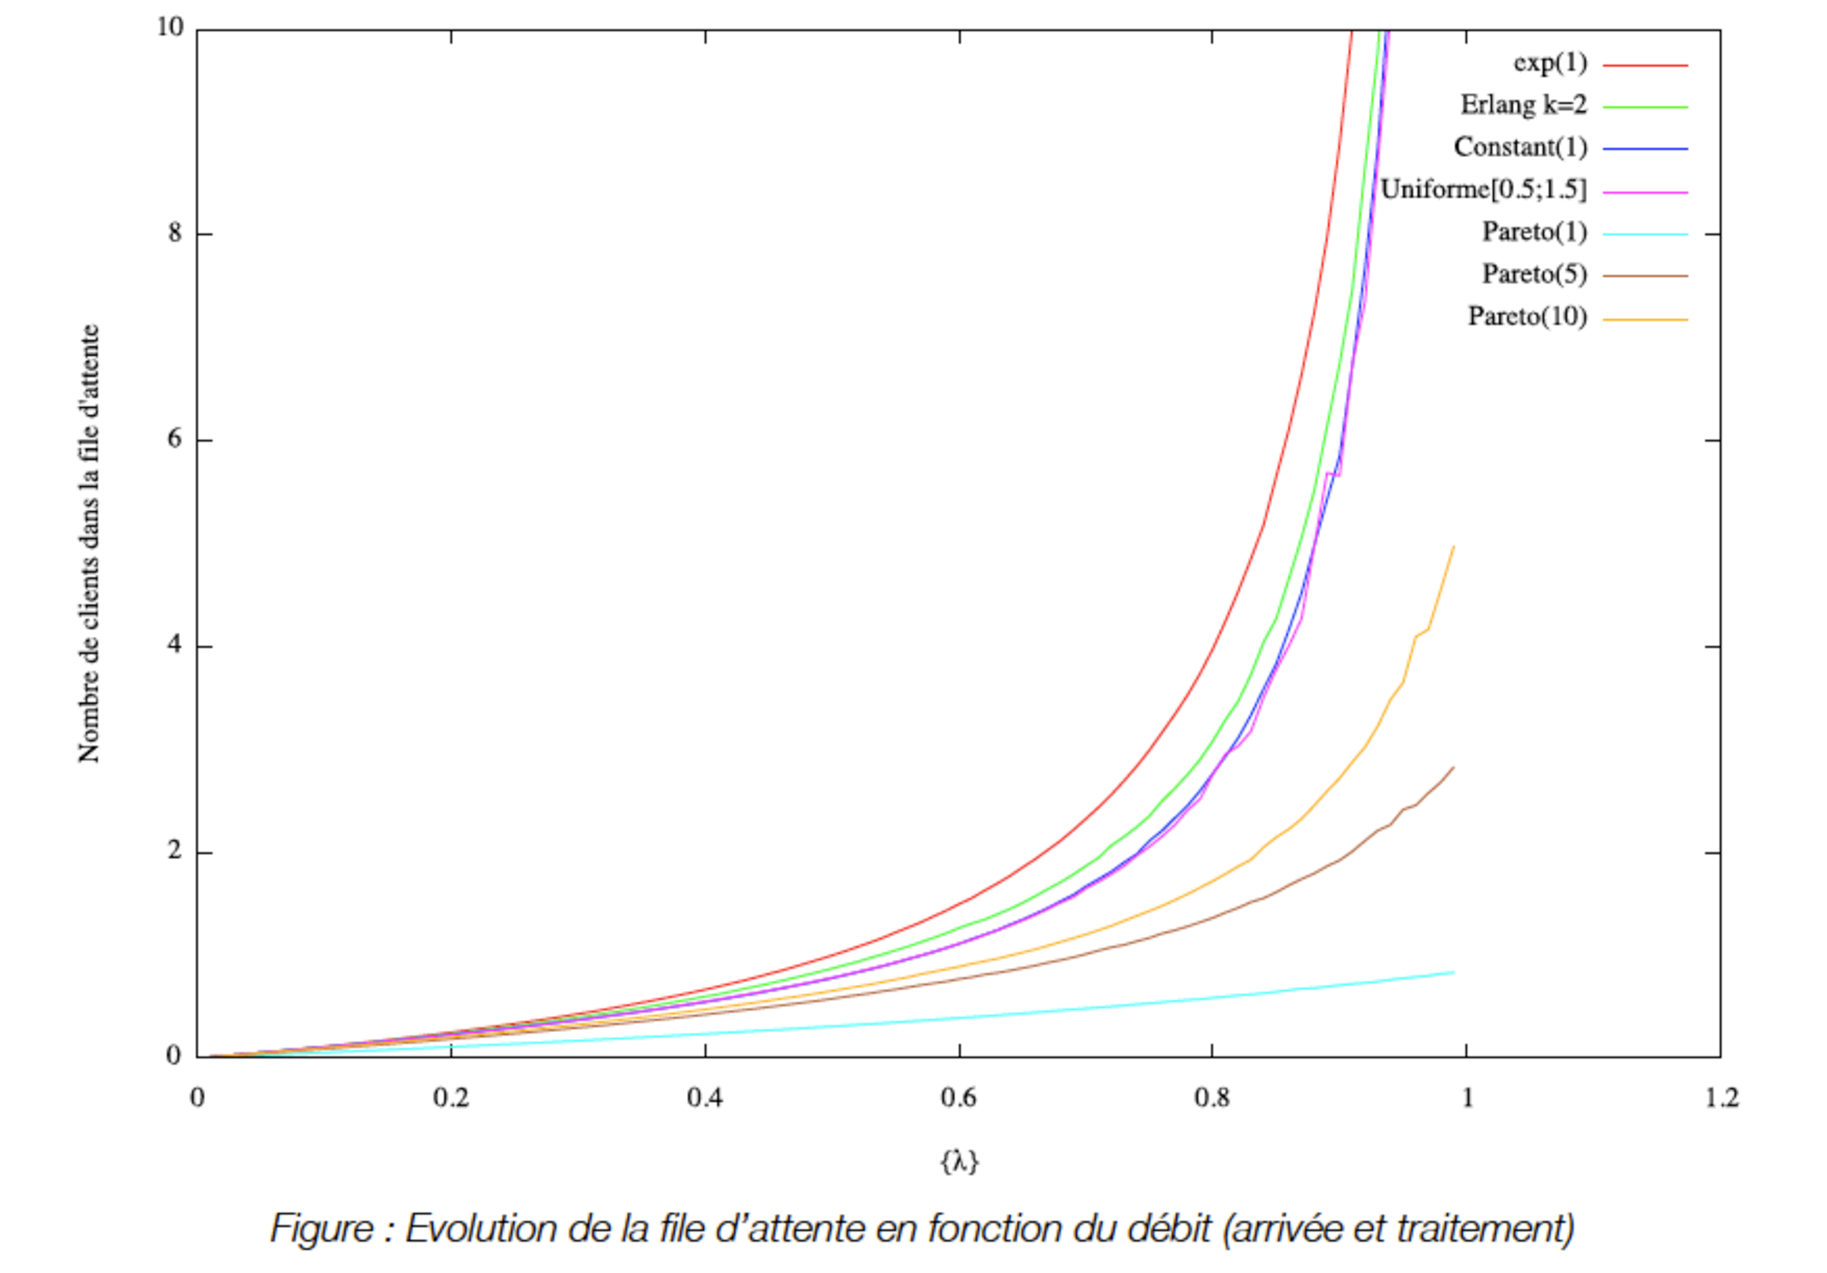
\includegraphics[width=0.8\textwidth]{Example10}
\end{center}
\end{frame}
\section[{\scshape Synthèse}]{{\scshape Synthèse }}
\begin{frame}{Synthèse}
\begin{alertblock}{Indications pour la conception d'une représentation graphique de données}
\begin{itemize}
\item Demander un effort minimal au lecteur;
%This is the most important characteristic of a good chart. Given two representations of the same data, it is usually easy to distinguish which one requires less effort. For example, direct labeling of curves is preferable to using a separate legend chart.
\item Maximiser l'information;
% There should be sufficient information to make a graph self-evident. Use key words instead of symbols since symbols require the reader remember the symbols. Make axis labels as informative as possible. For example, "Daily CPU Usage" rather than "CPU Usage". Include units on the labels "CPU Time in Seconds".
\item Minimiser  l'\textit{encre};
% Present as much information as possible with as little ink as possible. Too much unnecessary information clutters a chart.
\item Utiliser les conventions habituelles
%: Present what people expect. People expect the axis to be (0, 0). They expect the dependent variable to be on the y axis and the independent variable on the x axis. They expect linear scales, increasing from left to right and bottom to top, and all scale divisions to be equal. Departures are permitted but only when necessary.
\item Faire plusieurs représentations avant de choisir la meilleure.
\end{itemize}
\end{alertblock}
\begin{exampleblock}{Erreurs classiques à éviter}
\begin{itemize}
\item Trop d'objets graphiques
%: Curves with too many curves, bars or components should be avoided. A line chart should be limited to 6 lines. A bar chart should be limited to 10 bars. A pie chart should be limited to 8 components. Each cell in a histogram should contain at least 5 data points.
\item Confusion d'échelles
%: Combining unrelated charts to save space is not a good idea, especially if different variables use a different y axis.
\item Symboles à la place de texte
%: In the example, "2 jobs/sec" is a better label for a curve than "? = 2".
\item Information hors de propos
%: For example, grid lines are necessary only if the reader needs to read the chart very accurately.
\item Mauvais choix d'échelle/plages de valeurs
%: Don't just use the automatic scaling selected by a program like Excel. Override the default scaling if part of the range doesn't show any useful information.
\end{itemize}
\end{exampleblock}
\end{frame}
\begin{frame}{Synthèse}
\textbf{Toujours avoir à l'esprit :} Qui doit lire/interpréter le graphique et pourquoi ?

\begin{alertblock}{Principes}
\begin{itemize}
\item[] \textbf{\alert{Rasoir d'Occam}} Si deux représentations graphiques ont le même pouvoir d'information, choisir la représentation la plus simple.
\item[] \textbf{\alert{Principe de complétude (Dijkstra)}}  Quand on ne peut enlever un simple objet de la représentation graphique, alors elle est complète.
\item[] \textbf{\alert{Principe de bon sens}} Utiliser le niveau de sophistication adapté.
\end{itemize}
Adapté des livres 
\begin{itemize}
\item[1] Raj Jain. \textit{The Art of Computer Systems Performance Analysis : Techniques for Experimental Design, Measurement, Simulation, and Modeling}. John Wiley \& Sons, 1991.
\item[2] Jean-Yves Le Boudec. \textit{Performance Evaluation of Computer and Communication Systems}. EPFL Press, Lausanne, Switzerland, 2010.
\end{itemize}
\end{alertblock}
\begin{center}
{\large \textbf{Enfin}}: {\large \textbf{\alert{Le graphique doit être beau}}}
\end{center}
\end{frame}
\end{document}







